\documentclass[cover]{thesis}
% \documentclass[english]{famnit-thesis}       % For english version.
% \documentclass[cover]{famnit-thesis}         % Print the cover page.
% \documentclass[review]{famnit-thesis}        % The review version.
% \documentclass[english,cover]{famnit-thesis} % English version with the cover page.
% etc ...

% The bibliography is generated automatically through BibTex.
% Add the bibliography.bib file with all the bibtex entries.

% Import latex packages.
\usepackage{ccicons}
\usepackage{graphicx}
\usepackage{amssymb}
\usepackage{mathtools}
\usepackage{float}
\usepackage{standalone}
\usepackage{subcaption}

\graphicspath{ {./graphs/} }

% The basic thesis information.
\title
    {Nasprotniško spodbujevalno učenje v računalniških igrah za dva igralcaa}
    {Adversarial reinforcement learning in playing video games for two players}
    {Nasprotniško spodbujevalno učenje v računalniških igrah za dva igralca}

\author{Matic}{Stare}{M. Stare}
\studyprogram{Računalništvo in informatika}
\mentor{izr. prof. dr. Matjaž Kljun}{Assoc. Prof. Matjaž Kljun, PhD}
\date{avgust}{2023}

% Additional thesis information.
\comentor{asist. dr. Domen Šoberl}{Assist. Domen Šoberl, PhD}

% List of keywords in Slovene and English language.
\keywords
    {spodbujevalno učenje, Q-učenje, umetne nevronske mreže, arkadno učno okolje, algoritem DQN}
    {reinforcement learning, Q-learning, artificial neural network, The Arcade Learning Environment, DQN Algorithm}

% Abstract in Slovene and English language.
\abstract
{
    Področje strojnega učenja se v zadnjih letih pospešeno razvija. Del tega je tudi spodbujevalno učenje, ki se uporablja za učenje kompleksnih okolij, kot so na primer igre na simulaciji igralne konzole Atari 2600. Namen diplomske naloge je ugotoviti, kako uspešno se dva agenta spodbujevalnega učenja uspeta naučiti igrati igro Pong v nasprotniški postavitvi. S pomočjo programskega jezika Python in knjižnic PettingZoo ter Tensorflow smo implementirali algoritem globokega spodbujevalnega učenja (DQN) brez konvolucijskih plasti, saj smo namesto zaslonske slike igre izvedli vpogled v pomnilnik in od tam prebrali vhodne vrednosti. Za eksperimentalni del smo dve nevronski mreži pustili igrati igro Pong v nasprotniški postavitvi. Ugotovili smo, da po zadostnem številu učnih korakih nevronski mreži razvijeta napadalno strategijo, ki jima pomaga pri doseganju zadetkov. Rezultate smo prikazali na dva načina, in sicer z merjenjem dolžine posamezne epizode in s štetjem odbojev posameznega agenta v vsaki epizodi. 
}
{
    The field of machine learning has been rapidly advancing in recent years. Part of it includes reinforcement learning, which is used to learn complex environments, such as games on the Atari 2600 gaming console simulation. The purpose of this thesis is to determine how successful two reinforcement learning agents manage to learn the game of Pong in an adversarial setup. With the help of the Python programming language and libraries PettingZoo and TensorFlow we implemented the deep reinforcement learning algorithm (DQN) without convolutional layers, because we gained insight into the game's memory and read input values from there. For the experimental part, we let two neural networks play the game Pong in an adversarial setup. We found that after a sufficient number of learning steps, the neural networks develop an offensive strategy that helps them score points. We presented the results in two ways: by measuring the length of each episode and by counting the hits of the ball for each agent in every episode.
}

% The acknowledgments.
\acknowledgments
{   
    \noindent
    Zahvaljujem se svojima mentorjema za strokovno pomoč, spodbudo in potrpežljivost pri nastajanju tega diplomskega dela. 

    \noindent
    Hvala tudi vsem ostalim, ki so mi vsa leta pomagali pri študiju in mi stali ob strani.
}

% License page.
\licensepage
{
    ~\vfill\noindent
    To delo je ponujeno pod licenco \emph{Creative Commons Priznanje avtorstva --- Deljenje} pod
    enakimi pogoji 2.5 Slovenija (ali novejšo različico). To pomeni, da se tako besedilo, slike,
    grafi in druge sestavine dela kot tudi rezultati diplomskega dela lahko prosto distribuirajo,
    reproducirajo, uporabljajo, priobčujejo javnosti in predelujejo, pod pogojem, da se jasno
    in vidno navede avtorja in naslov tega dela in da se v primeru spremembe, preoblikovanja
    ali uporabe tega dela v svojem delu, lahko distribuira predelava le pod licenco, ki je enaka
    tej. Podrobnosti licence so dostopne na spletni strani \url{http://creativecommons.si/} ali na
    Inštitutu za intelektualno lastnino, Streliška 1, 1000 Ljubljana.

    \begin{center}
        \Huge\ccbysa
    \end{center}
    
    \medskip\noindent
    Izvorna koda diplomskega dela, njeni rezultati in v ta namen razvita programska oprema je
    ponujena pod licenco GNU General Public License, različica 3 (ali novejša). To pomeni,
    da se lahko prosto distribuira in/ali predeluje pod njenimi pogoji. Podrobnosti licence so
    dostopne na spletni strani \url{http://www.gnu.org/licenses/}.
}

% The list of abbreviations.
\abbreviation{ALE}{Arcade Learning Environment}
\abbreviation{DQN}{Deep Q-Network}
\abbreviation{MSE}{Mean Square Error}
\abbreviation{TanH}{Hyperbolic Tangent Function}
\abbreviation{ReLU}{Rectified Linear Unit}
\abbreviation{ADAM}{Adaptive Moment Estimation}

\begin{document}
% Thesis chapters.
\chapter{UVOD}

V zadnjih letih se je z razcvetom umetne inteligence področje strojnega učenja začelo pospešeno razvijati. Del tega je tudi spodbujevalno učenje~\cite{sutton2018reinforcement}, ki se osredotoča na učenje igralcev (agentov). Ti so postavljeni v okolje, v katerem morajo sprejemati odločitve, ki jih pripeljejo bližje cilju, kot odziv na izvedene akcije pa prejmejo nagrado oziroma kazen. Najbolj znana oblika spodbujevalnega učenja je Q-učenje, ki za ocenjevanje koristnosti akcij v nekem stanju uporablja Q-funkcijo. Na ta način se agent po zadostnem številu korakov lahko nauči precej dobro odločati, celo boljše od človeka. Ker je v večini učnih okolij različnih stanj in odločitev preveč, da bi Q-funkcijo hranili v obliki matrike, Q-funkcijo aproksimiramo z nevronsko mrežo. Ta se med treningom uči igralno strategijo, kasneje pa agent na njeni podlagi sprejema svoje odločitve.

Prva uspešna implementacija globokega spodbujevalnega učenja je bila predlagana leta 2013, ko je V. Minh s sodelavci z uporabo globoke nevronske mreže implementiral algoritem Q-učenja, ki se je lahko naučil igranja sedmih različnih iger v simulatorju igralne konzole Atari 2600~\cite{mnih2013playing}. Ena izmed njih je bila igra Pong, ki jo uporabljamo v tem diplomskem delu. Avtorji so uspeli nevronsko mrežo natrenirati do te mere, da je igro Pong lahko igrala bolje od človeka. Podobno smo v diplomskem delu poskusili tudi mi, le da smo uporabili različico igre Pong za dva igralca in trenirali dva agenta enega proti drugemu.

Cilj te diplomske naloge je ugotoviti, kako uspešno bi se dva agenta globokega spodbujevalnega učenja lahko naučila igrati igro Pong v nasprotniški postavitvi, tako da igrata eden proti drugemu. Delo zajema implementacijo Q-učenja v programskem jeziku Python z uporabo knjižnic TensorFlow~\cite{tensorflow2015} in Keras ter vzpostavitev arkadnega učnega okolja (ALE)~\cite{bellemare2013arcade} s pomočjo knjižnice PettingZoo~\cite{Terry_PettingZoo_Gym_for}, ki je razšititev knjižnice openAI Gymnasium~\cite{towers_gymnasium_2023} s podporo igranja igre za dva igralca, na katerem je igra simulirana. Nevronski mreži smo trenirali več dni, dokler način igranja obeh igralcev ni konvergiral k določeni strategiji. To pomeni, da vsako nadaljnje učenje ne bi prineslo nikakršnega napredka v uspešnosti igranja igre. Preizkusili in primerjali smo rezultate različnih globokih arhitektur nevronskih mrež in različnih vrednosti učnih parametrov, ki smo jih poskusili optimizirati.

V diplomskem delu bomo najprej predstavili teorijo spodbujevalnega učenja in Q-učenja ter opisali nevronske mreže, ki so potrebne za učenje računalniških igralcev. Sledi predstavitev implementacije, kar zajema opis posameznih komponent, ki so bile uporabljene in implementirane. Na koncu bomo predstavili rezultate dela in jih evalvirali. Kot zaključek sledi diskusija o možnih izboljšavah in nadaljnjem delu.

\chapter{GLOBOKO SPODBUJEVALNO UČENJE}
\section{SPODBUJEVALNO UČENJE}
\subsection{Kaj je spodbujevalno učenje}

Spodbujevalno učenje je področje strojnega učenja, ki se ukvarja z metodami agentnega učenja. Agent se v svojem okolju uči sprejemati odločitve, ki bi pripeljale do želenega cilja. Pri tem ga vodi funkcija nagrajevanja, od katere za dosežen cilj ali podcilj prejme nagrado. Agent se uči tako, da poskuša nagrado optimizirati, kar ob ustrezni definiciji funkcije nagrajevanja privede do odkritja uspešne strategije doseganja cilja~\cite{sutton2018reinforcement}. Ta princip se v vsakdanjem življenju pojavi vsakič, ko se želimo naučiti nečesa novega. V primeru učenja vožnje s kolesom bi spodbujevalno učenje lahko opisali takole: Na začetku še ne vemo, kakšna je naša najboljša strategija vožnje, zato z različnim zaporedjem akcij poskušamo poganjati pedala, usmerjati krmilo in ostati v ravnovesju. V prvih nekaj poskusih verjetno ne bomo uspešni, zato potrebujemo trening. Z vsakim poskusom nam gre bolje in kolo lahko vozimo vedno dlje. Zaradi uspešnosti dobimo občutek zadovoljstva, ki je pravzaprav nagrada za naše delo. Včasih pa se vseeno zgodi, da pademo. Zato je pomembno, da naše odločitve o izbiri akcij ustrezno prilagodimo tako, da se to v nadaljnje to ne bo več zgodilo. Po zadostni količini treninga znamo kolo že precej dobro voziti, kar pomeni, da se znamo v vsakem trenutku pravilno odločiti, kaj storiti, da ne pademo. Agent spodbujevalnega učenja na začetku v svojem okolju prav tako ne zna sprejemati odločitev, ki bi ga pripeljale do želenega rezultata. Med treningom se nato preko zaporedja poskusov in napak nauči sprejemati vedno boljše odločitve. Bolj kot je okolje kompleksno oziroma več kot je parametrov in akcij, več korakov agent potrebuje, da odkrije uspešno strategijo sprejemanja odločitev.

\subsection{Osnovni koncepti spodbujevalnega učenja}

Spodbujevalno učenje najlažje prikažemo z modelom na sliki~\ref{fig:rlmodel}. Osnovni koncepti spodbujevalnega učenja so \emph{agent}, \emph{okolje}, \emph{stanje}, \emph{nagrada} in \emph{akcija}. Vsakega izmed njih bomo na kratko predstavili.

\begin{figure}[H]
    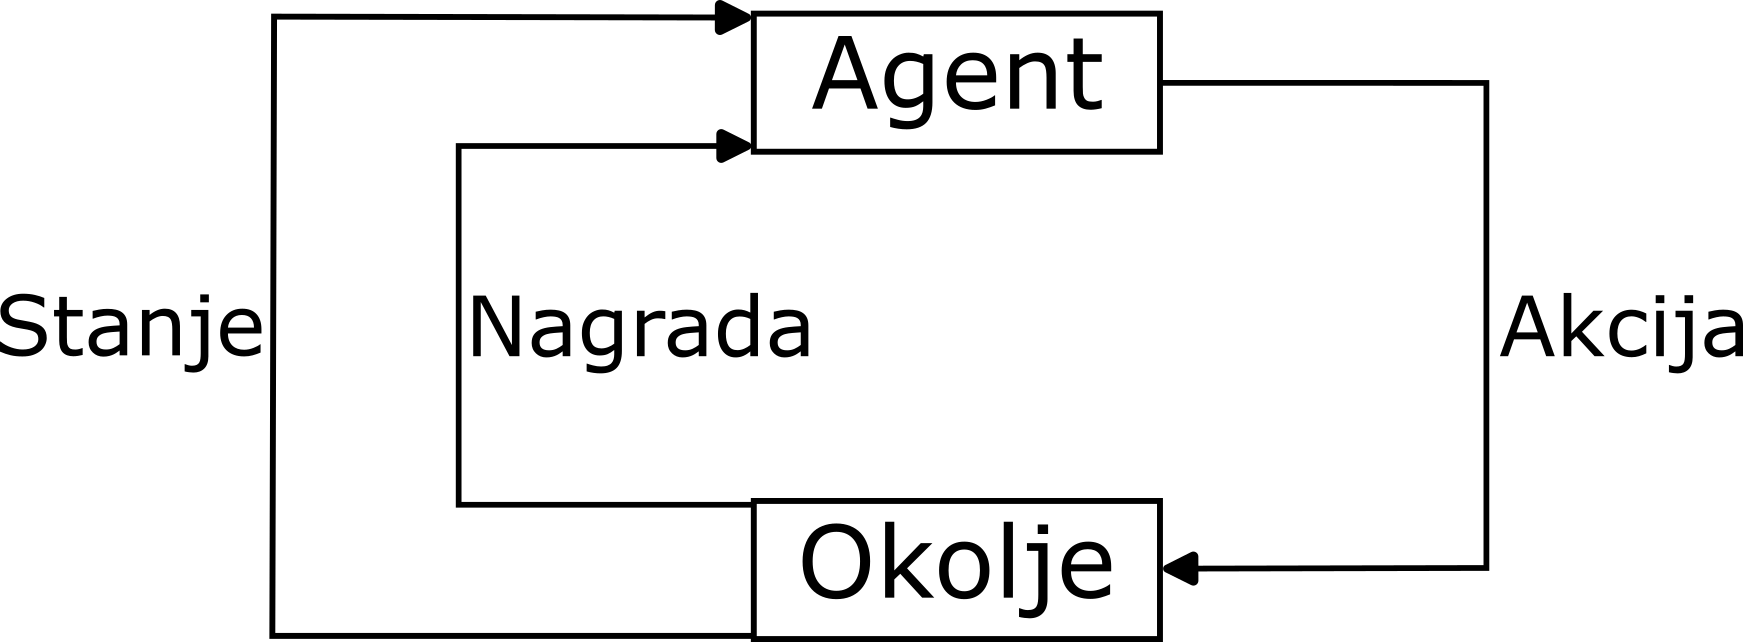
\includegraphics{RLmodel.png}
    \caption{Model spodbujevalnega učenja}\label{fig:rlmodel}
\end{figure}

\begin{itemize}
    \item \textbf{Agent} je entiteta, ki je postavljena v okolje in od njega pridobiva stanje, na podlagi katerega se odloči za naslednjo akcijo. Agent po vsaki izvedeni akciji prejme nagrado, ki je lahko pozitivna ali negativna. Koristnejša akcija prinese višjo nagrado, pri čemer negativna nagrada (kazen) lahko pomeni škodljivo akcijo.
    \item \textbf{Okolje} je prostor, v katerega je agent postavljen in na katerega s svojimi akcijami vpliva. Okolje je lahko zvezno ali diskretno.
    \item \textbf{Stanje} prikazuje trenutno situacijo agenta znotraj okolja oziroma njegovo konfiguracijo. Agent lahko stanje opazuje in iz njega zbira informacije, ki mu pomagajo pri izbiri akcij.
    \item \textbf{Nagrada} ja povratna informacija agentu po vsaki izvedeni akciji, ki mu sporoča kakovost njegove odločitve. Agentov cilj je maksimirati nagrado v vsakem koraku in s tem povečati skupno nagrado.
    \item \textbf{Akcija} je odločitev, ki jo agent sprejme v nekem stanju. Ta sproži prehod iz enega stanja v drugega.
\end{itemize}

V okolju spodbujevalnega učenja je agent seznanjen s trenutnim stanjem in na podlagi tega s pomočjo Q-funkcije, ki jo bomo predstavili v naslednjem poglavju~\ref{section:qlearning}, izbere in izvede naslednjo akcijo. S tem posodobi stanje in od okolja prejme nagrado, na podlagi katere posodobi Q-funkcijo. Tako Q-funkcija (ki jo v našem primeru aproksimiramo z nevronsko mrežo) počasi kovergira k neki sprecifični strategiji.

\subsection{Q-učenje}\label{section:qlearning}

Q-učenje je ena izmed najpogosteje uporabljenih izvedb spodbujevalnega učenja. Deluje tako, da agent vsakemu paru $(s,a)$ priredi vrednost \emph{Q}, ki 
pomeni kvaliteto izvedene akcije \emph{a} v stanju \emph{s}. Vrednost Q se izračuna po Bellmanovi enačbi:
\begin{equation}\label{eq:QfunkcijaEnacba}
    \underbrace{\text{New}Q(s,a)}_{\scriptstyle\text{Nova Q-vrednost}} =
    \overbrace{Q(s,a)}^{\scriptstyle\text{Q-vrednost}} +
    \mkern-25mu\underset{\text{Hitrost učenja}}{\underset{\Bigl|}{\alpha}}
    \mkern-25mu[\underbrace{R(s,a)}_{\scriptstyle\text{Nagrada}} +
    \mkern-35mu\underset{\text{Stopnja pojemanja}}{\underset{\Biggl|}{\gamma}}
    \mkern-60mu\overbrace{\max Q'(s',a')}^{\scriptstyle\substack{\text{Najvišja napovedana nagrada } \\ \text{glede na trenutno stanje}}}
    \mkern-20mu - 
    \mkern5mu Q(s,a)]
\end{equation}
Črka Q v besedi Q-učenje izhaja iz angleške besede \emph{Quality}, ki pomeni kvaliteta oziroma koristnost vsake akcije h končnem cilju. 

Osnovno Q-učenje poteka tako, kot je prikazano na sliki~\ref{fig:qtable}.
\begin{figure}[H]
    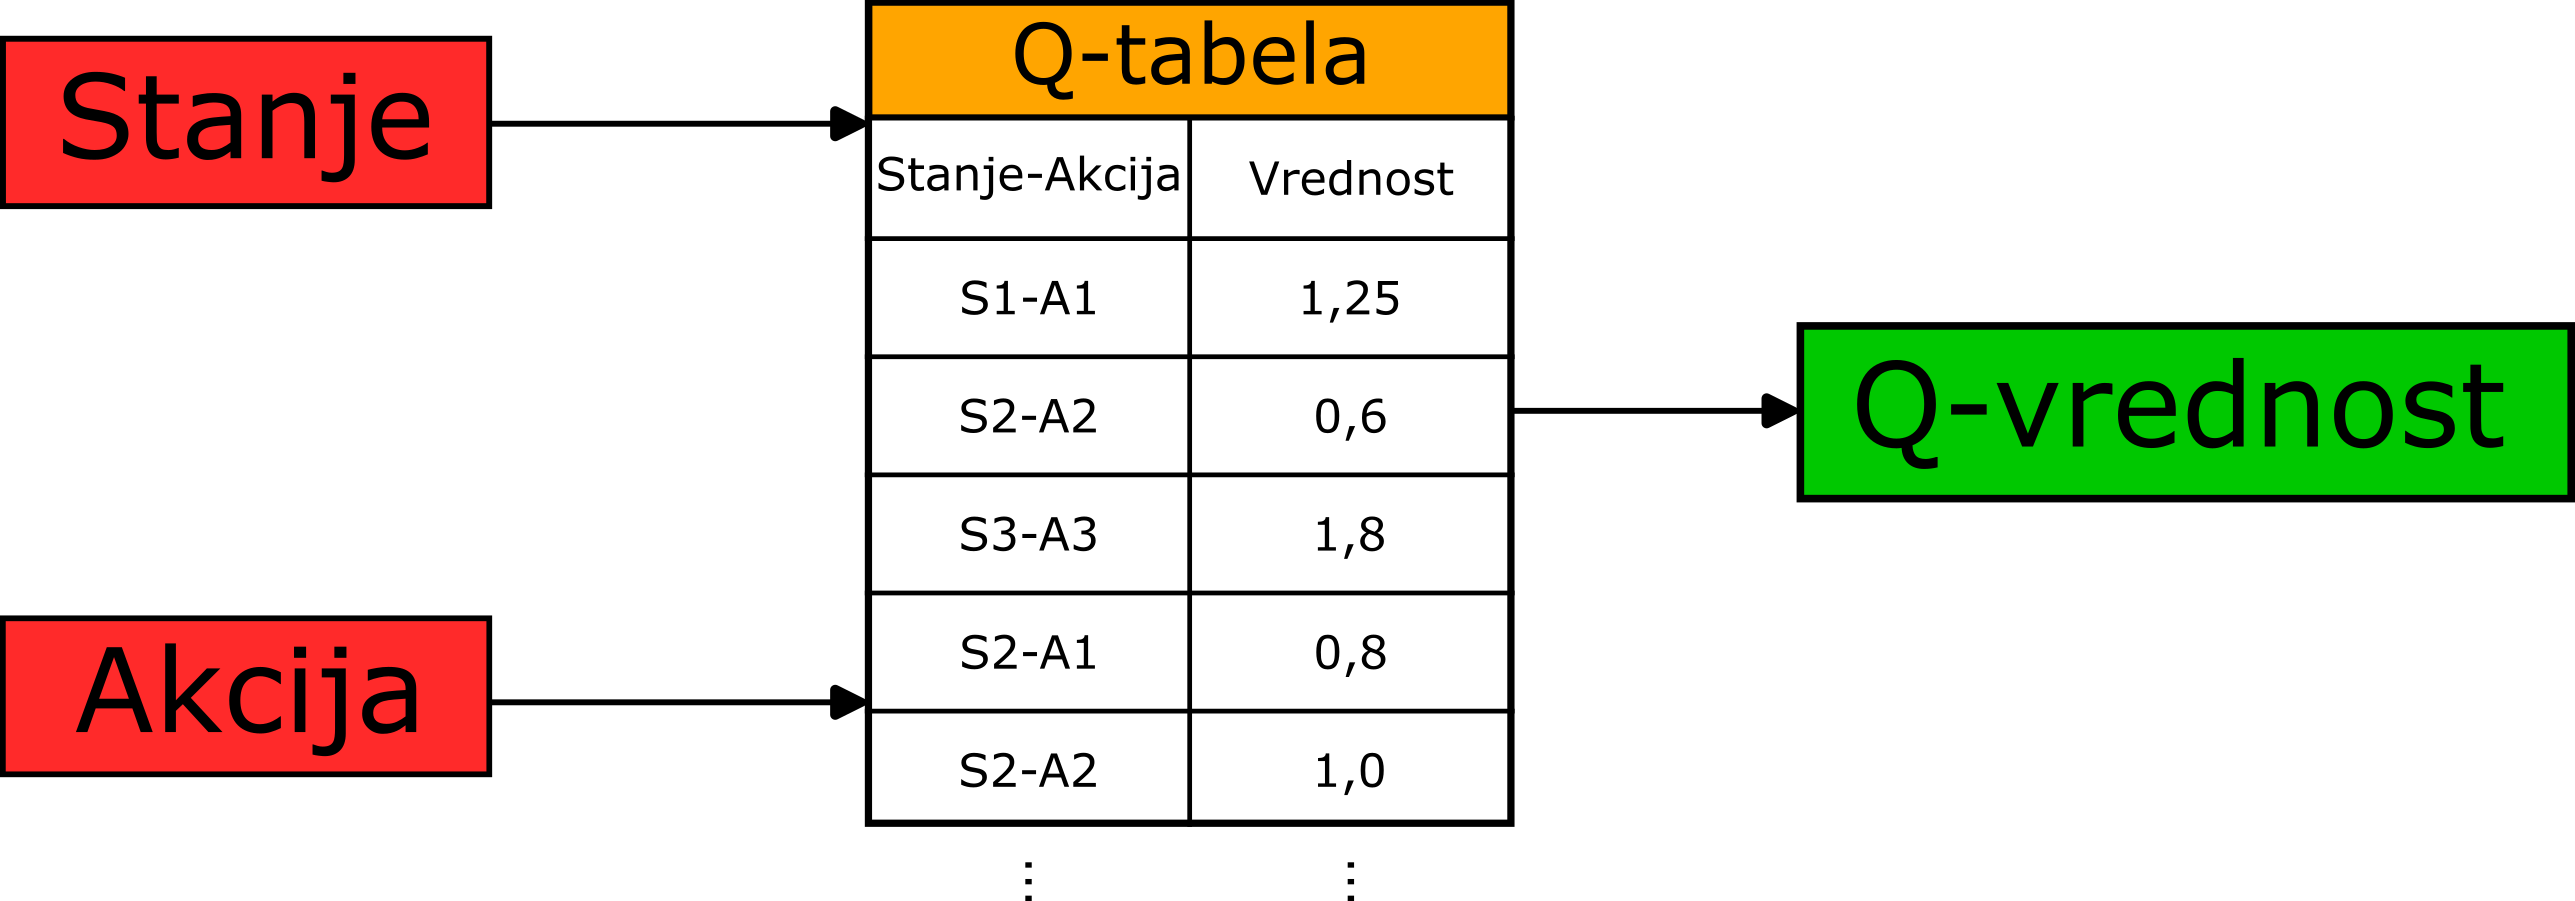
\includegraphics[width=\textwidth]{qtable.png}
    \caption{Q-učenje s pomočjo Q-tabele}\label{fig:qtable}
\end{figure}
Agent v vsakem koraku opazuje svoje trenutno stanje in vzame v obzir nabor vseh možnih akcij v tem stanju. S pomočjo Bellmanove enačbe~(\ref{eq:QfunkcijaEnacba}) nato izračuna pričakovano Q-vrednost ob izvedbi vsake od možnih akcij. Nato izvede akcijo z najvišjo Q-vrednostjo in na podlagi prejete nagrade posodobi vrednosti v Q-tabeli.

Algoritem Q-učenja lahko na kratko opišemo z naslednjo psevdokodo:
\begin{verbatim}        
    1. Inicializacija Q-vrednosti na 0.
    2. Za vsak korak znotraj epizode:
        2.1 Agent glede na trenutno stanje izbere akcijo z najvišjo
            Q-vrednostjo.
        2.2 Agent izvede akcijo in opazuje njen učinek (pridobi novo
            stanje in nagrado).
        2.3 Agent z uporabo enačbe (2.1) na podlagi prejete nagrade
            posodobi Q-vrednosti prejšnjega stanja in izvedene
            akcije.
    3. Evalvacija uspešnosti epizode.
    4. Ponovi koraka 1 in 2 za podano število epizod.
\end{verbatim}

\section{UMETNE NEVRONSKE MREŽE}
Z uporabo Q-tabele lahko implementiramo Q-učenje le v diskretnih domenah, zato v zveznih domenah preslikavo med pari stanje-akcija in Q-vrednostmi realiziramo preko realne funkcije. Učinkovit splošno-namenski aproksimator funkcij so nevronske mreže, ki lahko aproksimirajo, sicer z neko točnostjo, a ne glede na njihovo kompleksnost, poljubno matematično funkcijo. Točnost aproksimacije nevronske mreže je odvisna od velikosti njene arhitekture, števila iteracij preko učnih podatkov in narave učne množice podatkov. Bolj kot so podatki kompleksni, več plasti potrebujemo, da je aproksimacija funkcije točnejša.

Umetne nevronske mreže so sestavljene iz nevronov, ki so organizirani v plasti. Vsaka nevronska mreža je sestavljena iz ene ali več skritih plasti. Izhod posameznega nevrona je preko njih povezan na vhod naslednjega. Poznamo več vrst plasti umetnih nevronskih mrež. Prvi plasti rečemo vhodna, zadnji izhodna, vsem vmesnim plastem pa skrite plasti. Velikost vhodne plasti je neposredno povezana s številom vhodnih parametrov, saj potrebujemo toliko vhodnih nevronov, kot imamo vhodnih parametrov. Enako velja za izhodno plast, ki je velika toliko, kot potrebujemo izhodnih parametrov. Vmesne skrite plasti pa so odvisne od kompleksnosti učenja. Če želimo model naučiti nečesa bolj kompleksnega, potrebujemo več in večje skrite plasti. To pomeni, da nevronska mreža aproksimira matematično funkcijo treh neodvisnih spremenljivk, ki poljubno trojico realnih vrednosti enolično preslika v izhodno realno vrednost.

Primer nevronske mreže je prikazan na sliki~\ref{fig:NeuralNetwork}. Pri tem primeru je prva plast sestavljena iz treh nevronov, ki se preko dveh skritih plasti povezuje na en nevron izhodne plasti.
\begin{figure}[H]
    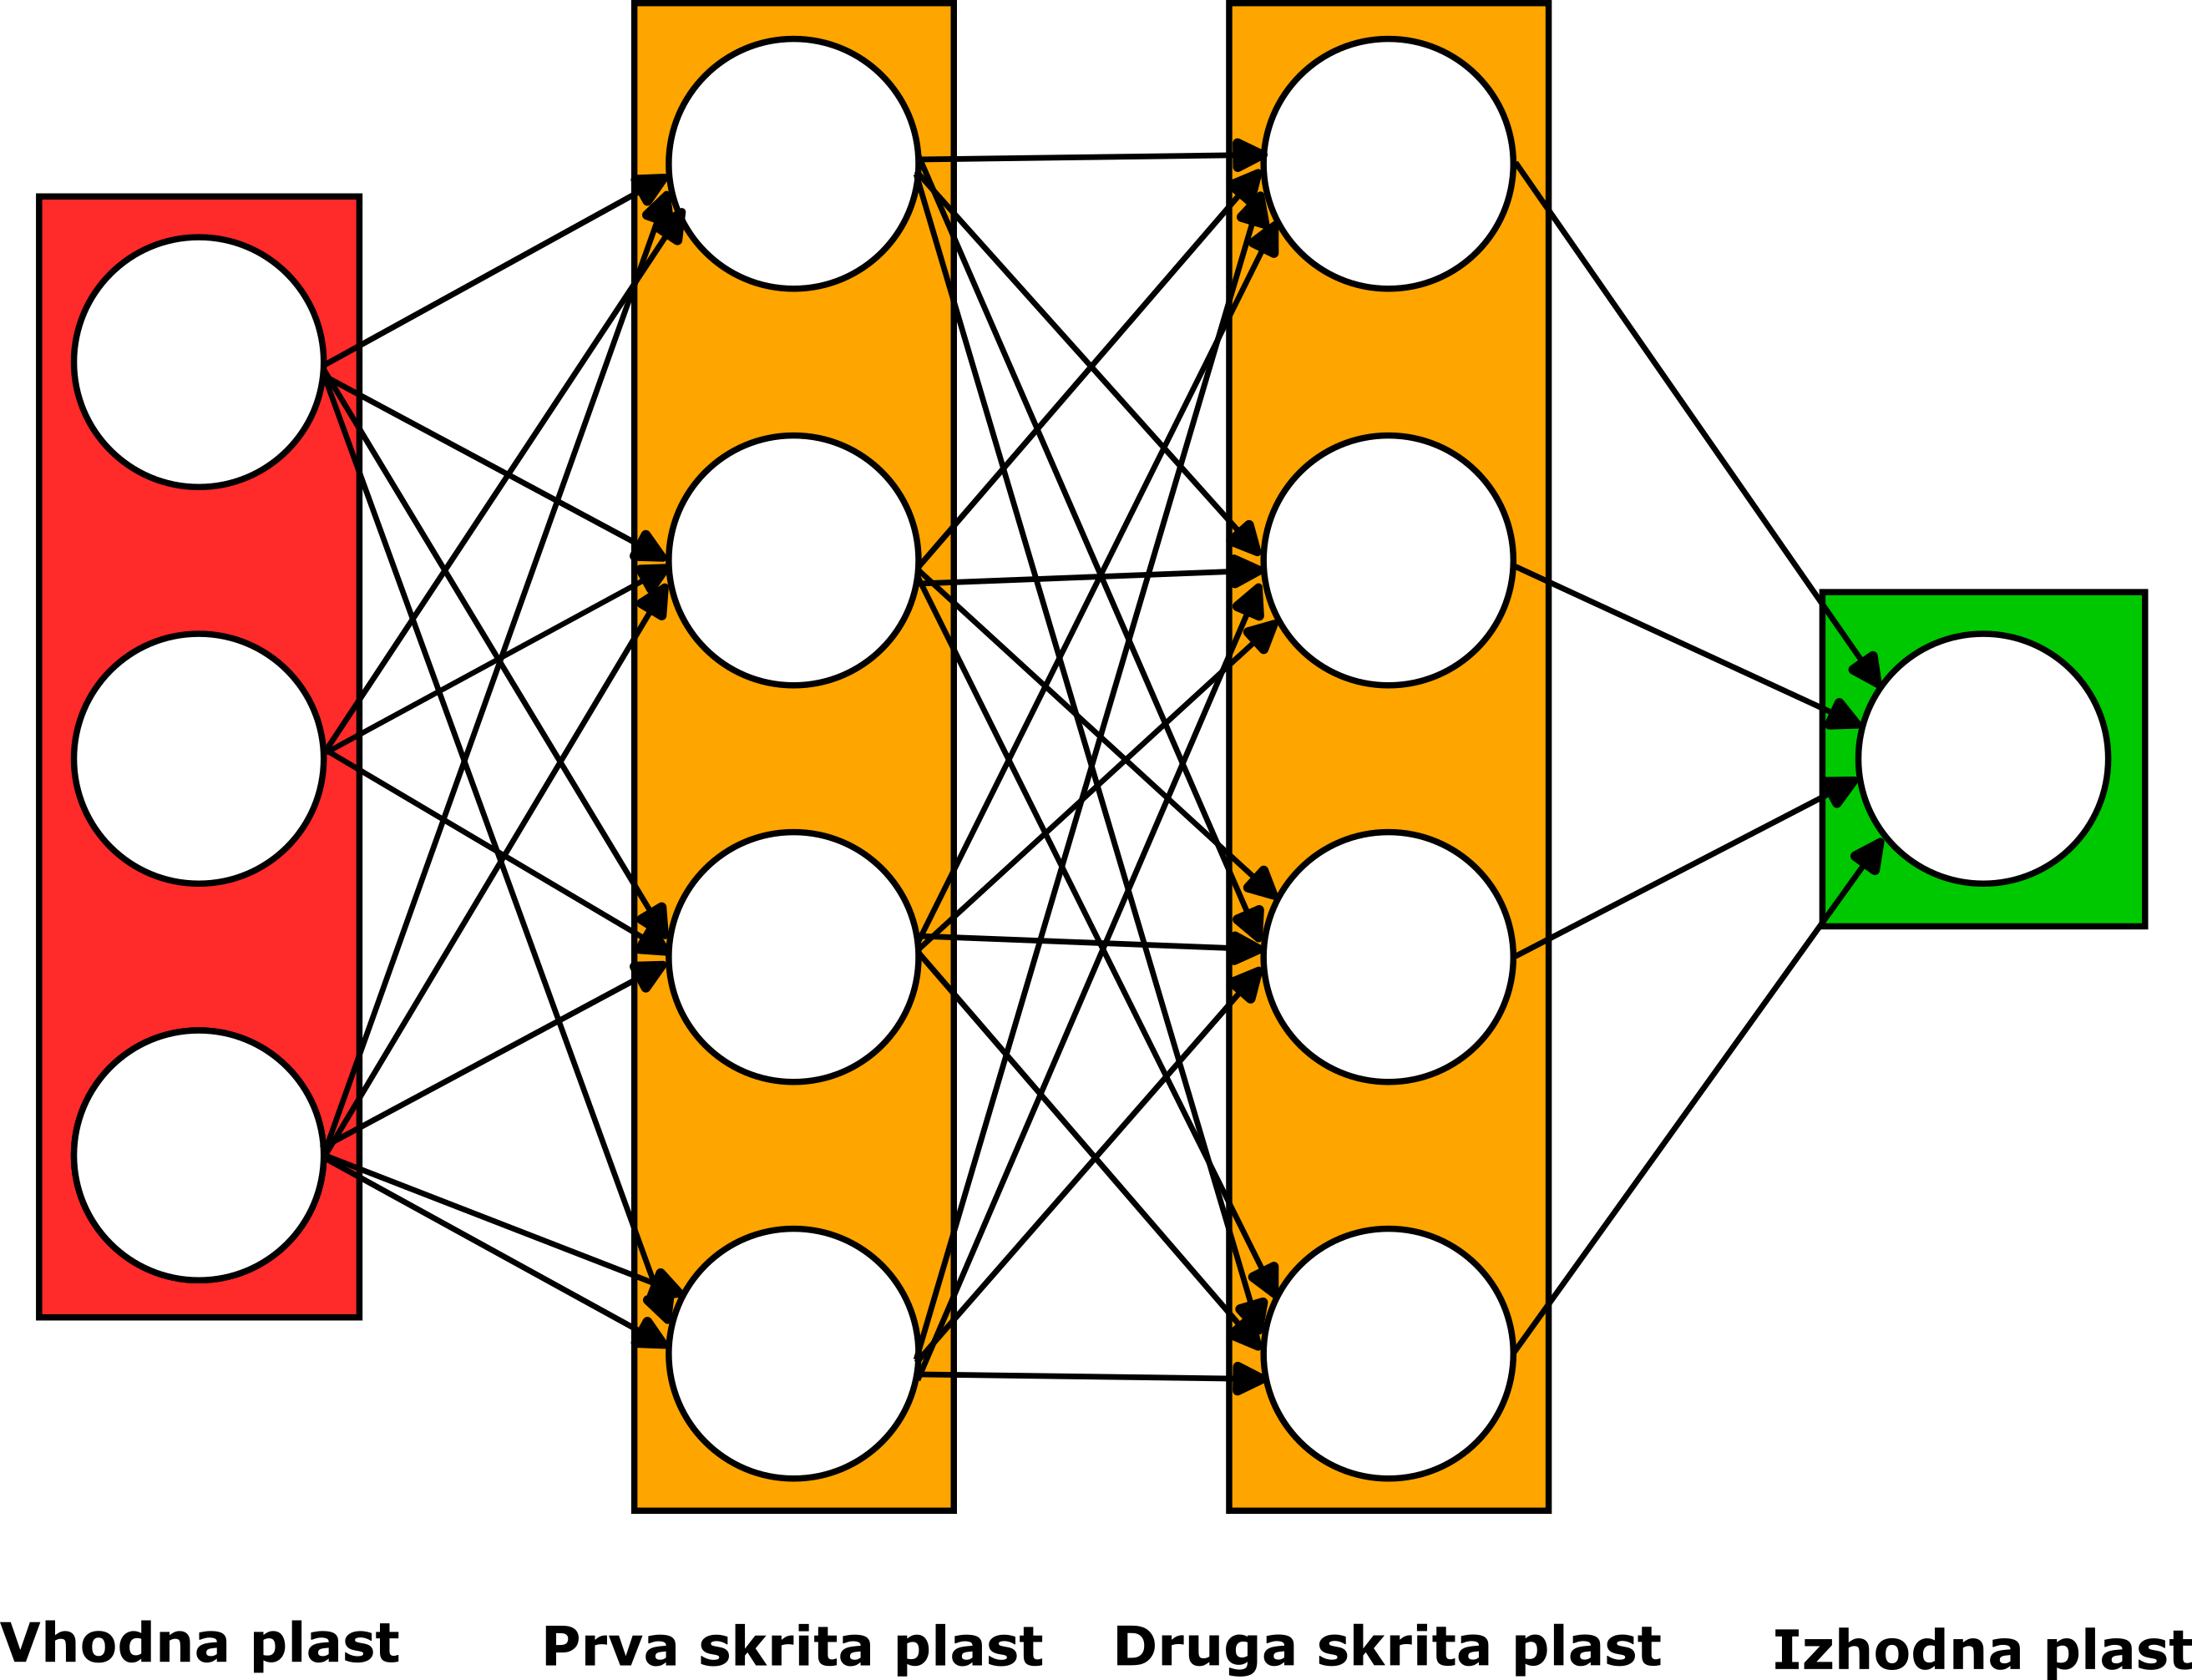
\includegraphics[width=\textwidth]{NeuralNetwork.png}
    \caption{Arhitektura napajalne nevronske mreže}\label{fig:NeuralNetwork}
\end{figure}

Glede na smer pretoka podatkov poznamo dve vrsti nevronskih mrež: napajalna (angl. \emph{feedforward}) in ponavlajoča se (angl. \emph{recurrent}). Pri prvi podatki tečejo od vhodne plasti enosmetno do izhodne. Za razliko od nje se pri drugi podatki lahko vračajo v predhodne plasti z namenom izboljšanja učenja. V diplomskem delu obravnavamo le napajalne nevronske mreže.

Delovanje nevronskih mrež lahko opišemo na sledeč način. V vsakem koraku dobi vhodne podatke, ki so navadno parametri okolja. Ti so podani vhodni plasti. Preko nevronskih povezav nato potujejo skozi skrite plasti proti izhodni plasti, pri čemer povezave med nevroni delujejo kot uteži. Na ta način nevronska mreža deluje pravzaprav kot preslikava ali funkcija, ki vhodne podatke preslika v izhodne. Na aktivacijo nevrona vpliva aktivacijska funkcija. Njen namen je v nevronsko mrežo vnesti nelinearnost, kar ji omogoča učenje tudi nelinearnih funkcij.

Vrednost posameznega nevrona izračunamo po naslednji enačbi:
\begin{equation}\label{eq:NeuronOutput}
    y = f\left(b + \sum_{i=1}^{n} (w_i \cdot x_i)\right)
\end{equation}
V tej enačbi $x_i$ predstavlja vhodne vrednosti nevrona, $w_i$ uteži vhodnih povezav, $b$ prag proženja, funkcija $f$ pa aktivacijsko funkcijo. Na sliki~\ref{fig:umetniNevron} je predstavljeno delovanje umetnega nevrona tudi vizualno.

\begin{figure}[H]
    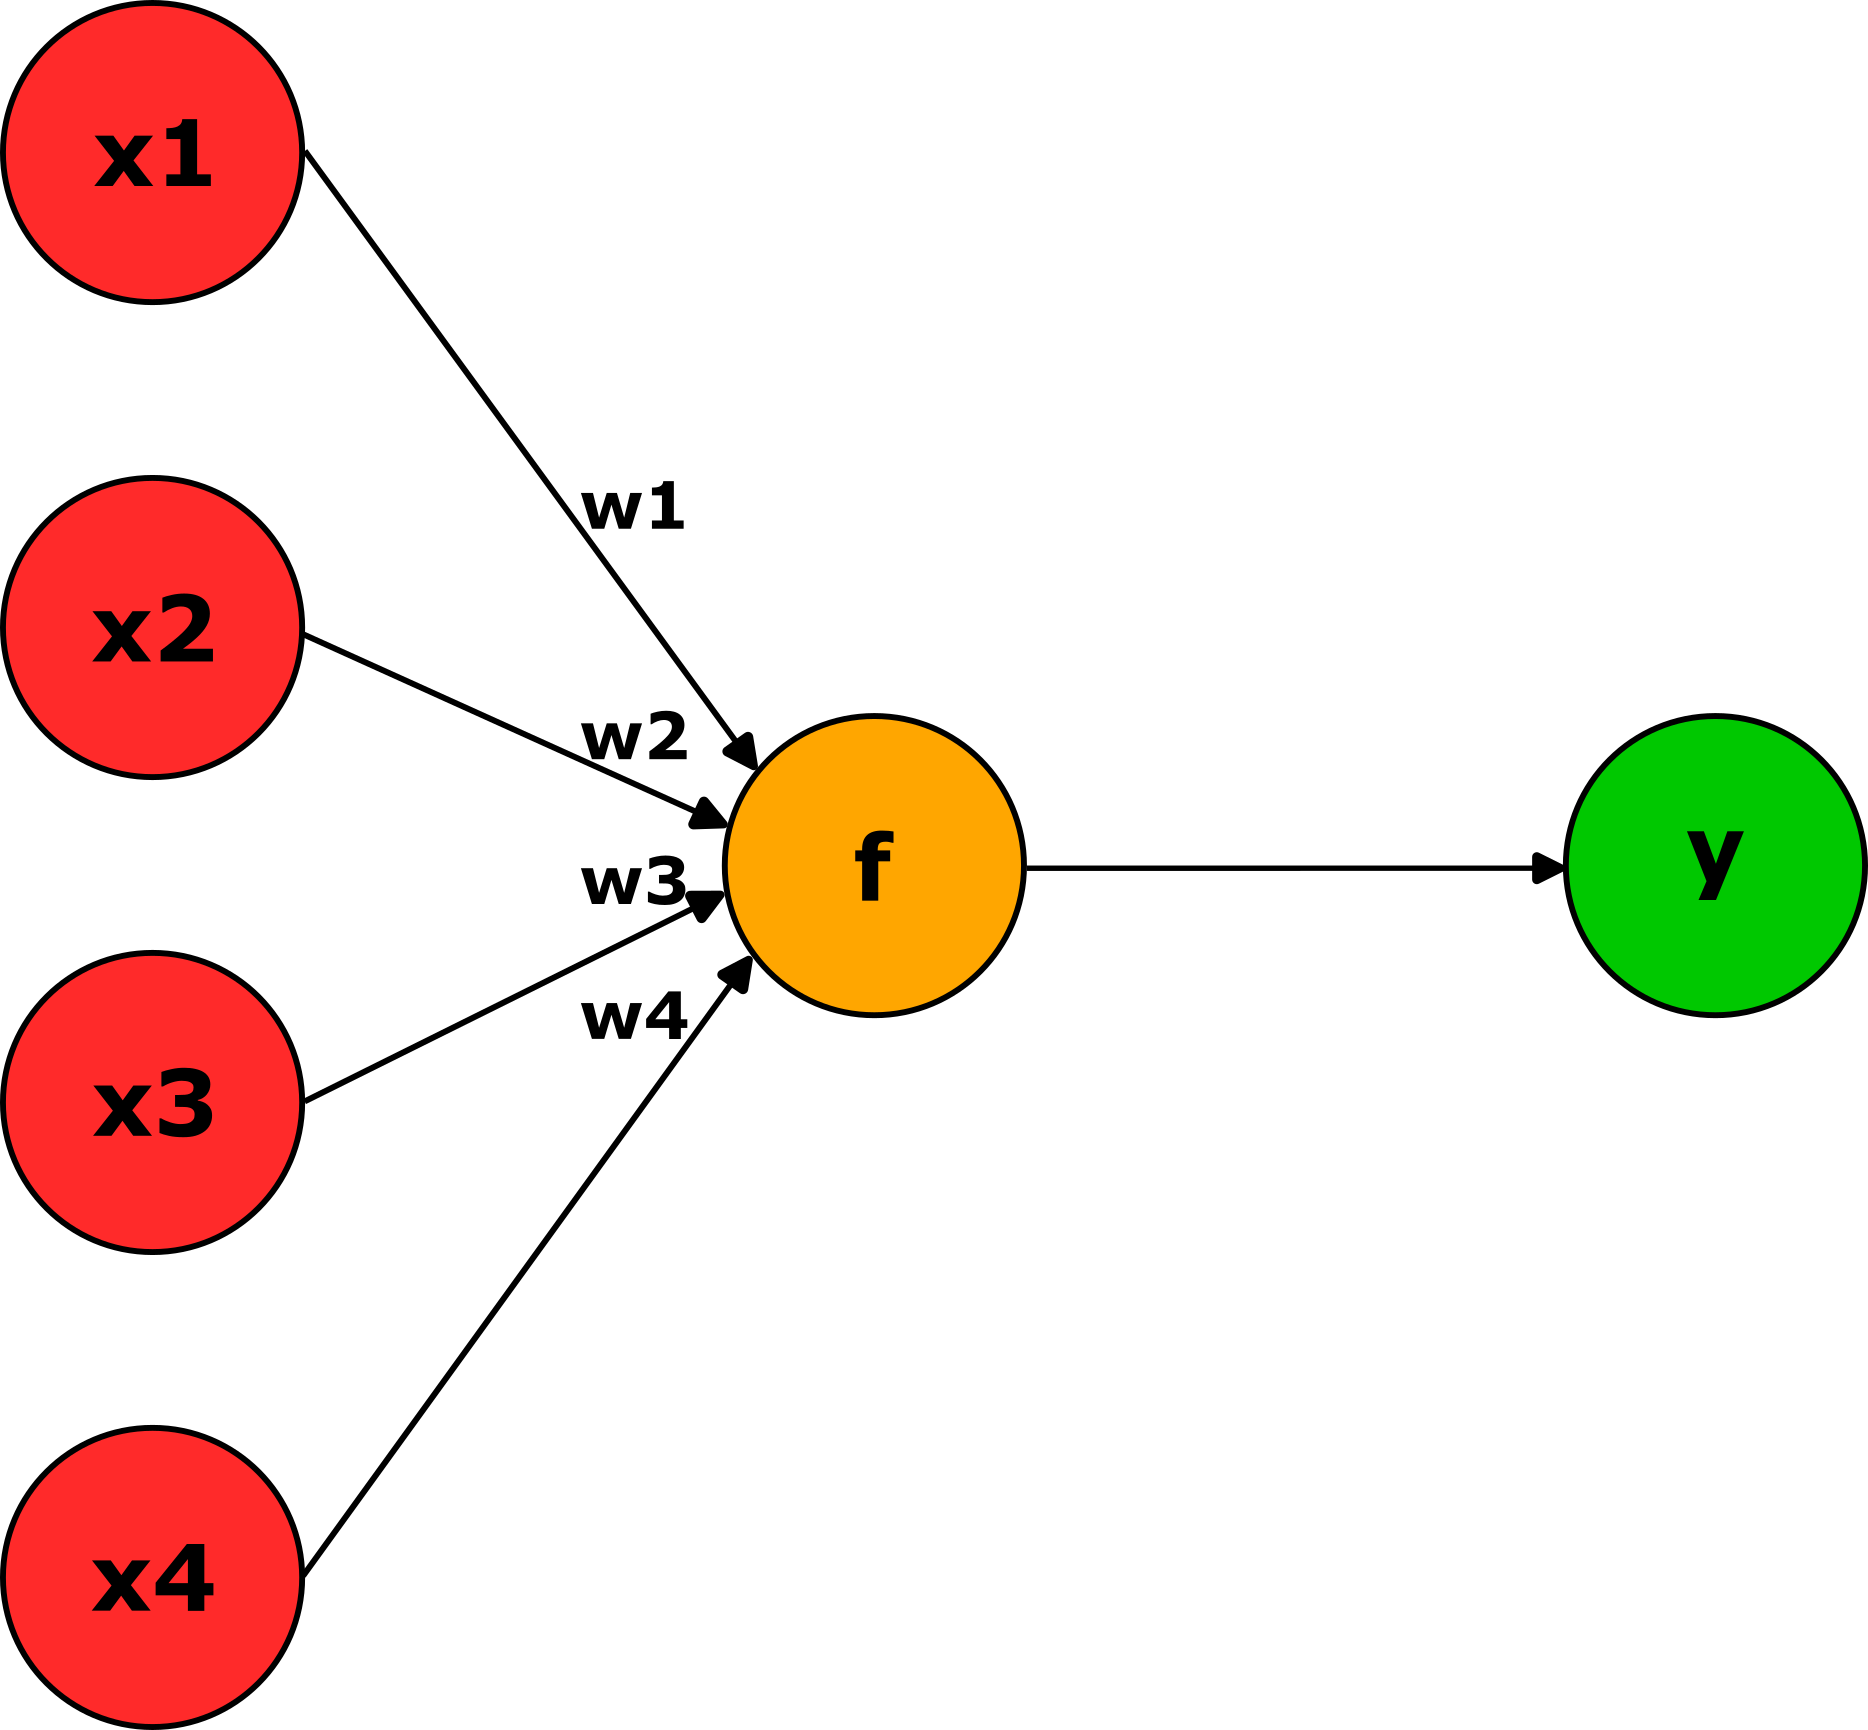
\includegraphics[width=\textwidth]{artificialNeuron.png}
    \caption{Delovanje umetnega nevrona}\label{fig:umetniNevron}
\end{figure}

Najpogosteje uporabljene aktivacijske funkcije so:
\begin{itemize}
    \item \emph{Sigmoidna funkcija} vhodne vrednosti preslika na interval (0,1), kar je uporabno predvsem pri binarni klasifikaciji.
    \item \emph{Funkcija TanH} je podobna sigmoidni funkciji le, da vhod preslika na interval (-1,1).
    \item \emph{ReLU} (Rectified Linear Unit) je aktivacijska funkcija, ki je zaradi svoje enostavnosti najpogosteje uporabljena pri globokih nevronskih mrežah. Zanjo je značilno, da vse negativne vhodne parametre preslika v 0, ostale pa pusti take kot so. To pomeni, da so v vsaki iteraciji aktivni le nenegativni nevroni.
\end{itemize}

\subsection{Učenje nevronskih mrež}

Učenje nevronskih mrež poteka iterativno. Na začetku se uteži nastavijo naključno. To pomeni, da je tudi matematična funkcija nevronske mreže na začetku naključna in pri napovedovanju izhodnih vrednosti dela relativno veliko napako. Potem se med učenjem ta funkcija in uteži prilagajajo in v vsakem koraku izboljšujejo. Funkcijo, ki določi napako nevronske mreže, imenujemo funkcija izgube (angl. \emph{loss function}). Pri učenju nevronskih mrež se pogosto uporablja povprečna kvadratna napaka (angl. \emph{Mean Square Error} ali MSE), ki smo jo uporabili tudi v tem diplomskem delu. MSE je definirana kot:
\begin{equation}\label{eq:MSE}
    MSE = \frac{1}{n} \sum_{i=1}^{n} (y_i - \bar{y})^2
\end{equation}
Glavni namen učenja nevronskih mrež je, da se to napako minimizira. Za minimizacijo napake se najpogosteje uporablja metoda vzvratnega razširjanja napake (angl. \emph{backpropagation}), ki deluje tako, da izhodno napako po vsakem izračunu izhodnih vrednosti širi po nevronski mreži od izhodne preko skritih to vhodne plasti. Med potjo uteži prilagodi tako, da se za trenutno aktivni primer izhodna napaka nekoliko zmanjša. Da se nevronska mreža na ta način bistveno izboljša, je potrebno postopek na velikem številu primerov več sto ali tisočkrat ponoviti. Ob ustrezno izbrani arhitekturi za dano domeno lahko pričakujemo, da bo nevronska mreža naučeno teorijo posplošila tudi na primere, ki jih s to metodo ni obdelala ter dajala pravilne napovedi tudi za primere, ki se v učni množici niso pojavili.

Postopek učenja nevronske mreže lahko opišemo na sledeči način:

\begin{verbatim}        
    1. Vhodna plast nevronske mreže sprejme enega ali več
        učnih primerov.
    2. Učni nevroni aktivirajo vhodne nevrone glede na trenutno
        nastavljene vhodne uteži.
    3. Vhodni nevroni glede na trenutno vrednost aktivirajo
        skrite plasti, te pa izhodno plast.
    4. Funkcija izgube izračuna napako izhodne plasti.
    5. Algoritem vzvratnega razširjanja uravnava uteži od izhodnih
        proti vhodnim plastem tako, da zmanjšuje napako.
    6. Zgornje korake ponavljamo, dokler ne dosežemo želene točnosti
        izhodnih vrednosti.        
\end{verbatim}

\subsection{Uporaba nevronskih mrež pri Q-učenju}

Globoko Q-učenje se od klasičnega spodbujevalnega Q-učenja razlikuje po tem, da Q-tabelo zamenjamo z umetno nevronsko mrežo. To je primerno v situacijah, ko je okolje preveč kompleksno, da bi hranili vsa možna stanja v tabeli, zato odločitve aproksimiramo z umetno nevronsko mrežo. Prvi znani algoritem globokega Q-učenja DQN~\cite{mnih2013playing} deluje na principu konvolucije, kar pomeni, da kot vhod prejme kar surovo zaslonsko sliko, iz katere konvolucijske plasti nevronske mreže izluščijo informativne atribute. V našem primeru konvolucijske plasti izpustimo in atribute stanja podamo neposredno, kar bistveno zmanjša prostor stanj in pospeši proces učenja. To smo storili, ker dodajanje drugega učečega agenta v igro, kjer se je v predhodnih DQN implementacijah učil en sam agent, bistveno poveča prostor stanj, ki ga je potrebno preiskati, naš čas in naši razpoložljivi viri pa so bili omejeni.

Vsaka agentova akcija proizvede novo izkušnjo, ki jo agent shrani v svoj pomnilnik izkušenj.
Ta izkušnja je sestavljena iz štirih komponent: trenutno stanje, izvedena akcija, prejeta nagrada in novo stanje (kot posledica izvedene akcije). To pomeni, da vsak zapis v pomnilniku izkušenj vsebuje dve zaporedni stanji.

Ko se v pomnilniku izkušenj nabere dovolj izkušenj za vsaj en sveženj (angl. \emph{batch}), nevronska mreža prične z učenjem. V našem primeru je velikost svežnja konstantna, in sicer 32 izkušenj. Po vsaki izvedeni akciji agent novo pridobljeno izkušnjo doda v pomnilnik izkušenj, iz njega pa naključno izbere 32 izkušenj, nad katerimi nevronska mreža izvede en učni korak. To pomeni, da vsakemu koraku igranja sledi učni korak nad naključno izbranim svežnjem 32-ih preteklih izkušenj. Ta pristop k učenju smo prevzeli od algoritma DQN.

Algoritem globokega Q-učenja lahko predstavimo z naslednjo psevdokodo:
\begin{verbatim}        
    1. Inicializiraj pomnilnik izkušenj.
    2. Inicializiraj igralno in tarčno umetno nevronsko mrežo
       z naključnimi utežmi.
    3. Ponovi naslednje korake za M epizod:
        3.1 Inicializiraj začetno stanje igre.
        3.2 Glede na vrednost stopnje preiskovanja izberi naključno
            akcijo ali s pomočjo tarčne nevronske mreže.
        3.3 Izvedi akcijo in pridobi nagrado ter opazuj naslednje
            stanje.
        3.4 Pridobljeno izkušnjo shrani v pomnilnik izkušenj.
        3.5 Iz pomnilnika izkušenj izberi sveženj k naključnih
            izkušenj in z uporabo Bellmanove enačbe izračunaj
            dejanske Q-vrednosti.
        3.6 Izvedi učni korak igralne nevronske mreže nad svežnjem
            izračunanih dejanskih Q-vrednosti.
        3.7 Če je že preteklo določeno število korakov, prepiši uteži
            igralne nevronske mreže v tarčno nevronsko mrežo.
\end{verbatim}

Slika~\ref{fig:deepQLearning} prikazuje preslikavo stanja v akcijo, ki naj bi jo agent v danem stanju izvedel. Nevronska mreža vsaki akciji priredi Q-vrednost, algoritem pa nato izbere najvišje ocenjeno akcijo. Učenje nevronske mreže poteka tako, da za izbrani sveženj izkušenj z uporabo Bellmanove enačbe~(\ref{eq:QfunkcijaEnacba}) izračunamo dejanske Q-vrednosti vsake akcije in nad temi dejanskimi vrednostmi izvedemo učni korak s povratnim širjenjem napake.

\begin{figure}[ht]
    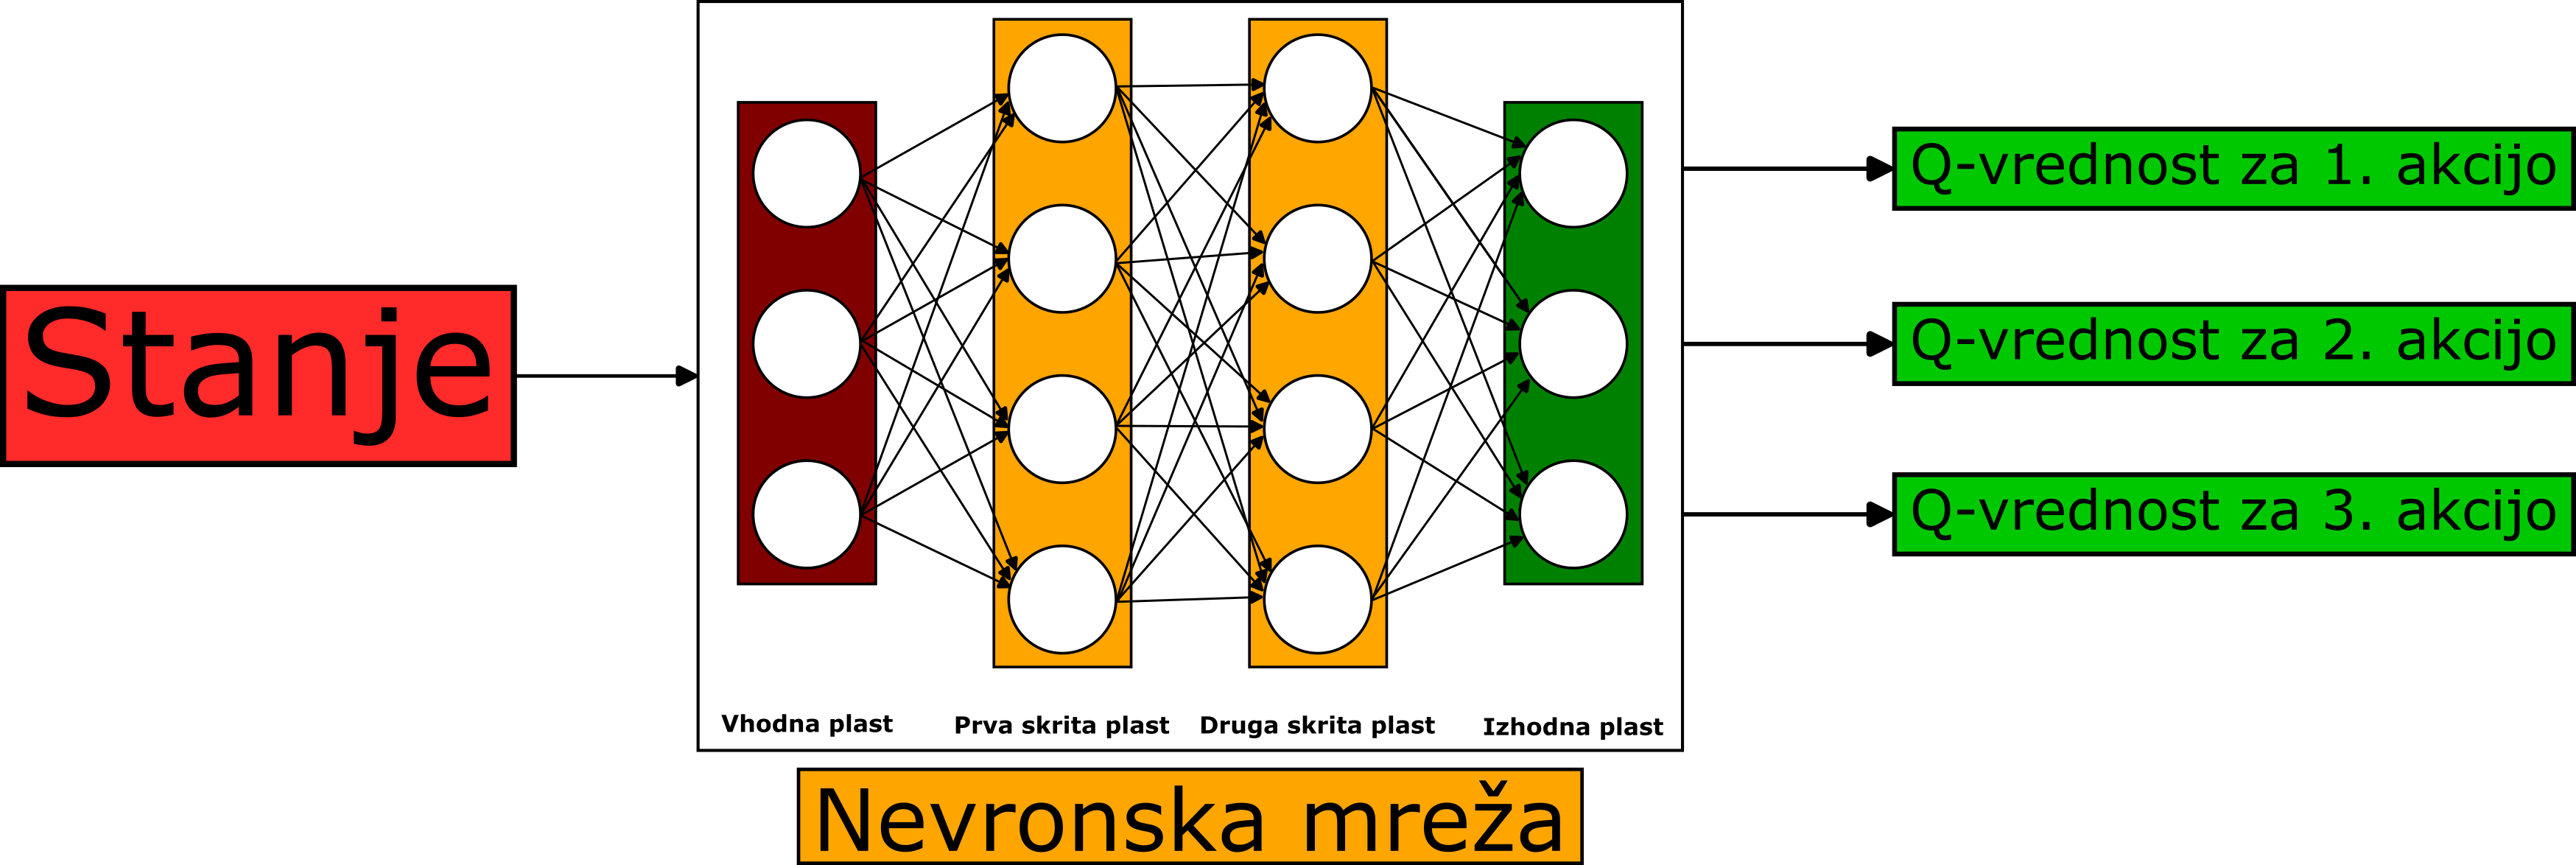
\includegraphics[width=\textwidth]{deepQLearning.png}
    \caption{Q-učenje s pomočjo nevronske mreže}\label{fig:deepQLearning}
\end{figure}

\chapter{IMPLEMENTACIJA}

Algoritem spodbujevalnega učenja smo implementirali v programskem jeziku Python, s pomočjo knjižnic Tensorflow~\cite{tensorflow2015} in Keras~\cite{chollet2015keras}. Ker smo potrebovali podporo za dva igralca, smo za simulacijo igre Pong namesto osnovnega okolja Gymnasium~\cite{towers_gymnasium_2023} uporabili njegovo ovojnico z imenom PettingZoo~\cite{Terry_PettingZoo_Gym_for}. Vse omenjene knjižnice smo namestili z uradnim Pythonovim upraviteljem paketov Pip~\cite{pypi}.

\section{ARKADNO UČNO OKOLJE}

Arkadno učno okolje je ogrodje, ki simulira igralno konzolo Atari 2600 in nam omogoča enostaven razvoj agentov za igranje poljubne igre, ki jo ta konzola podpira~\cite{bellemare2013arcade}. Na voljo je več različnih iger. Za potrebe te diplomske naloge se bomo osredotočili na igro Pong. V vsakem koraku je agentu na voljo 6 različnih akcij. Te smo še okrnili in uporabili le 3 najpomembnejše, in sicer akcija 1 (serviraj žogo), akcija 2 (premakni se gor) in akcija 3 (premakni se dol). Simulator v vsakem koraku prejme agentovo akcijo, jo izvede in kot izhod vrne zaslonsko sliko, ki predstavlja trenutno stanje igre, ter nagrado. Ker je podatkov v zaslonski sliki veliko, smo namesto nje za učenje nevronske mreže izvedli vpogled v pomnilnik igre, iz katerega smo prebrali položaj igralne žoge, ki je podana z dvema koordinatama $x$ in $y$, ter položaj obeh igralcev, ki sta podana le s koordinato $y$. Imamo torej 4 vhodne parametre.

Slika~\ref{fig:pong} prikazuje zaslonsko sliko igre Pong.

\begin{figure}[H]
    \centering
    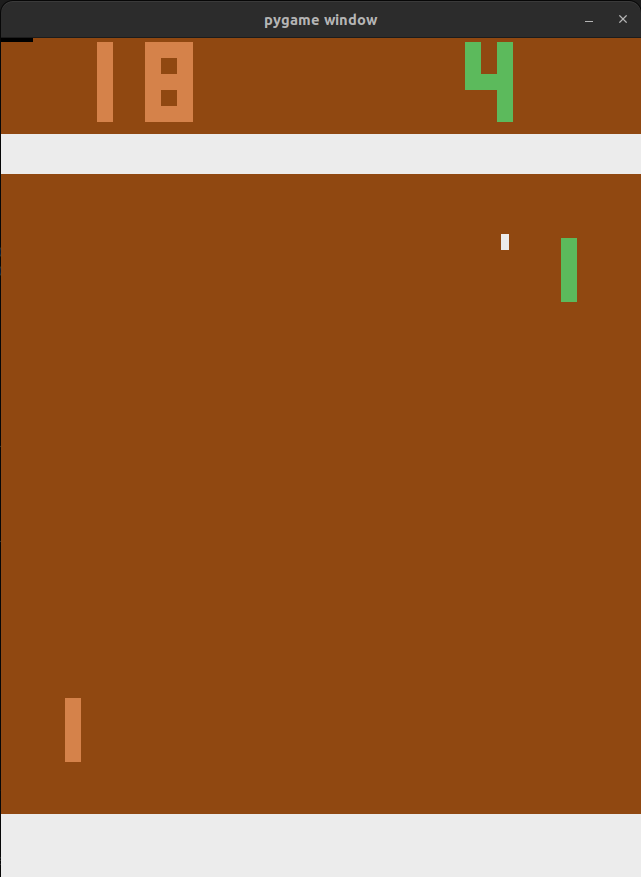
\includegraphics[width=7cm]{pong.png}
    \caption{Zaslonska slika igre Pong}\label{fig:pong}
\end{figure}

Na tej sliki lahko vidimo prvega igralca (oranžne barve) na levi, drugega igralca (zelene barve) na desni in igralno žogo (bele barve). Na vrhu lahko opazujemo tudi rezultat trenutne igre. V tem primeru levi igralec vodi z rezultatom 18 proti 4.

Ker smo v tej nalogi želeli izvesti nasprotniško učenje dveh agentov, smo potrebovali simulator, ki podpira igranje za 2 igralca, kar nam je omogočila knjižnica PettingZoo. Simulator dodeli nagrado le ob danem (vrednost nagrade 1) ali prejetem (vrednost nagrade -1) zadetku, kar pomeni, da je velika večina prejetih nagrad enaka 0. Ob razširitvi igre na dva igralca se je izkazalo, da je ob takšnem sistemu nagrajevanja učenje prepočasno, zato smo implementirali nov sistem dodeljevanja nagrad. Za dosežen zadetek smo agentu podelili 10 točk, za prejet zadetek -10 točk, za uspešen odboj žoge 1 točko in za vse ostalo 0 točk. S tem smo agenta nagradili tudi v primeru, ko je žogo odbil, kar v prejšnjem sistemu ni bilo zaznano.

\section{GLOBOKO Q-UČENJE}

V našem primeru je agent postavljen v okolje, kjer mora na podlagi štirih vhodnih podatkov --- pozicija obeh igralcev in žoge --- pravilno napovedati najboljšo naslednjo akcijo. V našem primeru agent lahko izbira med tremi akcijami. Te so: serviranje žoge po prejetem zadetku, premik loparja gor in premik loparja dol. Ker poskušamo dva igralca naučiti igrati igro enega proti drugemu, potrebujemo za vsakega izmed njih svojo instanco algoritma spodbujevalnega učenja. Da se učenje ne bi zataknilo v nekem lokalnem maksimumu, smo uporabili koncept algoritma DQN, ki namesto le ene nevronske mreže uporabi dve, in sicer igralno (angl. \emph{policy}) in tarčno (angl. \emph{target}) nevronsko mrežo. Igralna nevronska mreža je tista, na kateri se v vsakem koraku izvaja učenje. Tarčna nevronska mreža pa za igralno mrežo zaostaja določeno število korakov. S tem dosežemo stabilnejše učenje.

\begin{figure}[H]
    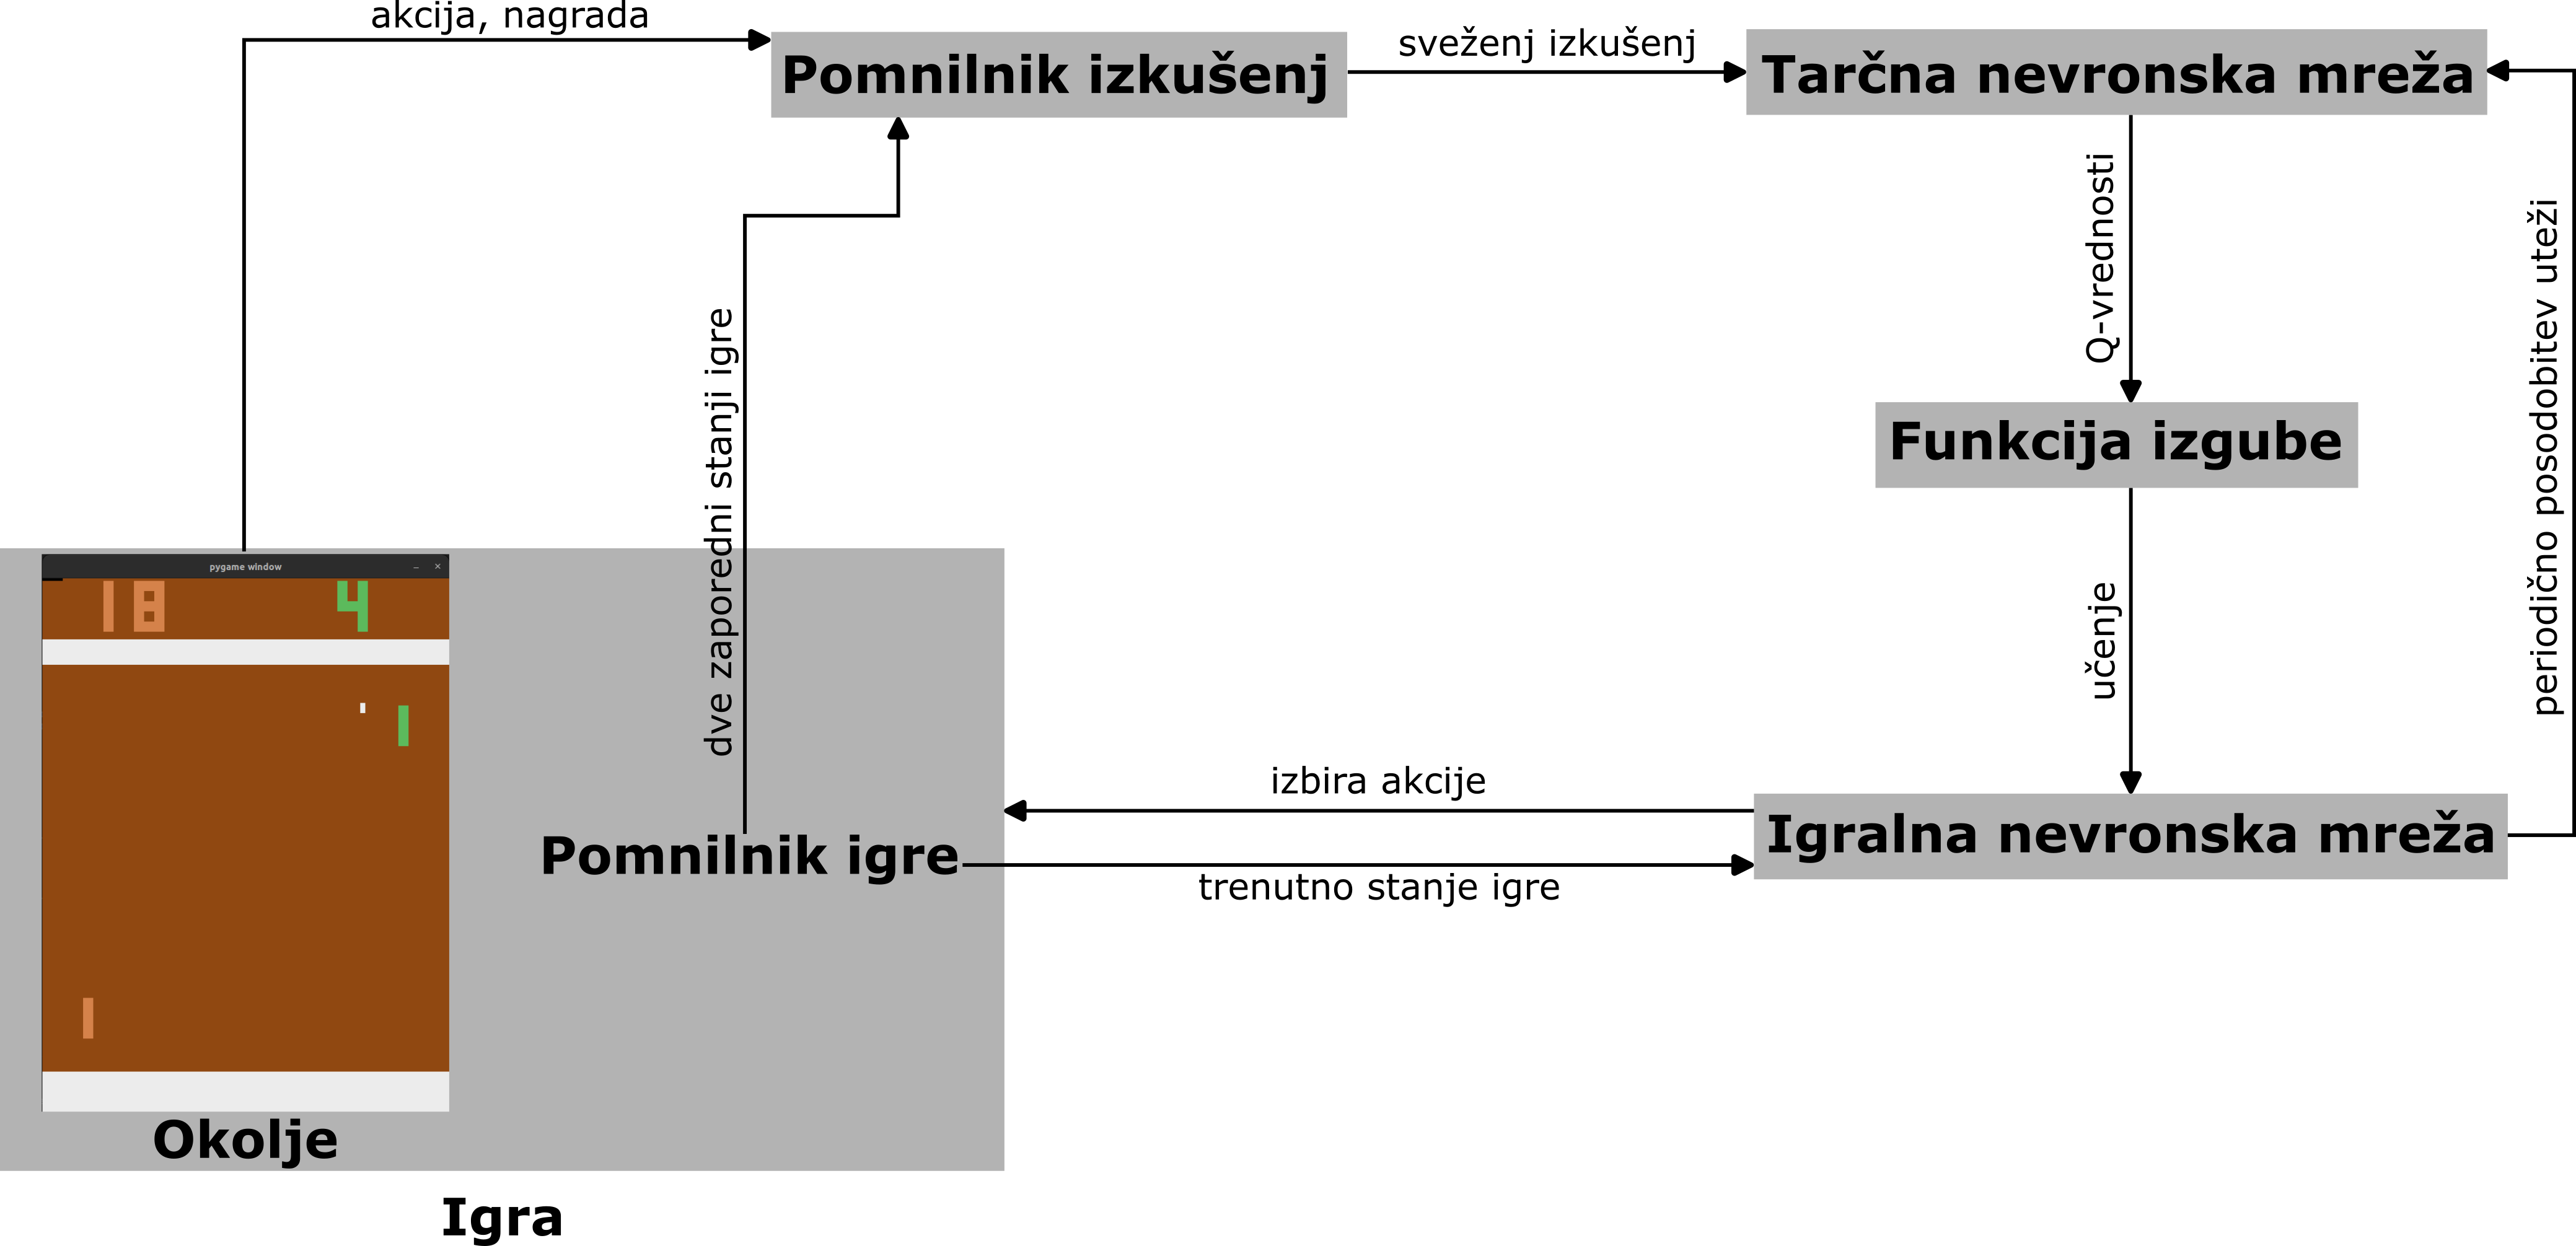
\includegraphics[width=\textwidth]{NNgameScheme.png}
    \caption{Arhitektura globokega spodbujevalnega učenja po vzoru algoritma DQN za učenje igre Pong}\label{fig:gameScheme}
\end{figure}
Na sliki~\ref{fig:gameScheme} je prikazana shema poteka igre Pong in učenja tarčne in igralne nevronske mreže. V vsakem koraku se nova izkušnja shrani v pomnilnik izkušenj. Iz njega se potem izbere sveženj 32 naključnih izkušenj, ki se jih servira tarčni nevronski mreži. Ta napove Q-vrednosti, za vsako izmed njih. Potem se s pomočjo funkcije izgube to preda igralni nevronski mreži, ki na prejetih vrednostih izvede korak učenja. V vsaki iteraciji igre pa igralna nevronska mreža od okolja prejme tudi trenutno stanje igre, na podlagi katerega se mora odločiti za najboljšo akcijo.

\section{ARHITEKTURA NEVRONSKE MREŽE}\label{section:nnarchitecture}

Izbira arhitekture umetne nevronske mreže za globoko spodbujevalno učenje je odvisna od kompleksnosti okolja in števila akcij, ki se jih mora agent naučiti. Če je okolje enostavno, je bolje izbrati enostavnejšo arhitekturo, saj se te lahko učijo hitreje. Po drugi strani pa se enostavna arhitektura ne more naučiti zahtevnejših strategij v kompleksnejših okoljih.

Pri izbiri ustrezne arhitekture oziroma velikosti vseh skritih plasti nevronske mreže smo imeli kar nekaj težav, saj smo začeli s premajhnimi skritimi plastmi. To je pripeljalo do tega, da se mreži nista naučili dovolj, da bi začeli uspešno odbijati žogo. Preizkusili smo več različnih konfiguracij in na koncu izbrali naslednjo:
\begin{verbatim}        
    1. Vhodni sloj: 4 nevroni
    2. Prvi skriti sloj: 256 nevronov
    3. Drugi skriti sloj: 2048 nevronov
    4. Izhodni sloj: 3 nevroni
\end{verbatim}
Velikost vhodne in izhodne plasti je določena z dimenzijo stanj in številom akcij. Velikost prve skrite plasti smo nastavili na 256 nevronov, druge pa na 2048 nevronov. To je omogočilo, da je arhitektura dovolj velika, da se po zadostnem številu učnih korakov mreži naučita odbijati žogo. Za izhodno plast smo uporabili linearno aktivacijsko funkcijo, na vseh ostalih pa funkcijo ReLU. Vse plasti nevronske mreže so polno povezane, kar pomeni, da je vsak nevron povezan z vsemi nevroni predhodnje plasti.

\section{PREISKOVANJE PROSTORA STANJ}

Na začetku so uteži v nevronski mreži inicializirane na naključne vrednosti, kar pomeni, da agent sledi naključni igralni strategiji, kar lahko vodi (in pogosto tudi vodi) k ponavljanju istega zaporedja akcij. Agent tako ne pridobiva novih izkušenj in se zato ne more ničesar naučiti. To rešimo tako, da vpeljemo naslednji princip. Najprej definirajmo pojem stopnje preiskovanja (angl. \emph{exploration rate}) kot $\varepsilon \in [0,1]$, kjer 0 pomeni popolno izkoriščanje, 1 pa popolno preiskovanje. Pred vsako izbiro akcije sistem izbere naključno realno število med 0 in 1. Če je naključno izbrano število med 0 in 1 večje ali enako vrednosti $\varepsilon$, agent izbere akcijo na podlagi trenutno naučene strategije, sicer pa izbere naključno akcijo. Vrednost $\varepsilon$ na začetku nastavimo na 1, kar pomeni, da agent na začetku izbira le naključne akcije, z vsako naslednjo epizodo pa vrednost $\varepsilon$ nekoliko zmanjšamo. Tako se agent vedno bolj opira na naučeno igralno strategijo. Vrednost $\varepsilon$ vedno obdržimo nekoliko nad 0, saj s tem v igro vnesemo nekaj variabilnosti, še posebej, če so začetni pogoji vedno enaki. Najnižja stopnja preiskovanja, ki smo jo uporabili tako med treniranjem kot med igranjem, je bila $\varepsilon = 0\text{,}1$. To pomeni, da je bilo vedno vsaj 10 \% akcij izbranih naključno.

\chapter{REZULTATI}\label{section:results}

\section{IGRA ZA ENEGA IGRALCA}

Svojo implementacijo globokega spodbujevalnega učenja smo najprej preizkusili na igri Pong za enega igralca, pri čemer lopar drugega igralca upravlja algoritem, ki so ga sprogramirali avtorji igre Pong. Gre za preprost algoritem, ki predvsem sledi gibanju žogice. Tako smo se prepričali, da naš učni algoritem deluje pravilno. Uporabili smo sledečo arhitekturo nevronske mreže, ki se je v takšni igralni postavitvi izkazala najbolje:
\begin{verbatim}        
    1. Vhodni sloj: 4 nevroni
    2. Prvi skriti sloj: 64 nevronov
    3. Drugi skriti sloj: 512 nevronov
    4. Izhodni sloj: 3 nevroni
\end{verbatim}

Preiskusili smo tudi nevronske mreže z arhitekturo skritih plasti 16/128, 32/256 in 128/1024, vendar so te dosegale precej slabše rezultate. Eksperimentirali smo tudi z vrednostjo $\varepsilon$. Na koncu smo se odločili, da $\varepsilon$ do 1 milijona učnih korakov pada linearno od 1 proti 0,1 ter tam ostane do konca učenja. Določili smo tudi število začetnih korakov, med katerimi agent še ne izvaja učenja, ampak izvaja naključne akcije in s tem polni pomnilnik izkušenj. Za to smo določili 50.000 začetnih korakov.

Učenje smo pustili teči 72 ur na strežniku s procesorjem Intel Xeon, ki ima frekvenco jedra 3,5GHz. V tem času je agent odigral 1325 epizod, kar je približno 5 milijonov učnih korakov.

\begin{figure}[H]
    \centering
    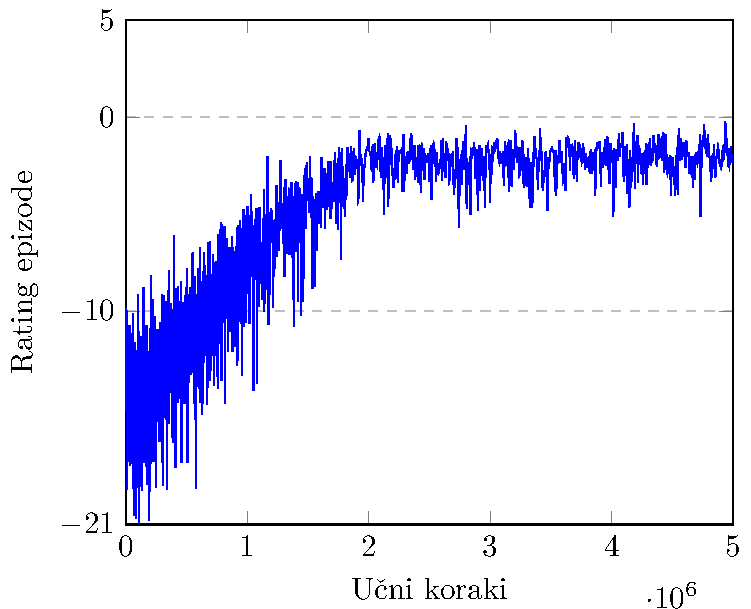
\includegraphics{fig1.pdf}
    \caption{Graf učenja igre Pong za enega igralca}\label{fig:singleRating}
\end{figure}

Na sliki~\ref{fig:singleRating} je prikazan \emph{rating} igranja igre Pong za enega igralca proti vgrajenem računalniškem igralcu. Rating predstavlja oceno uspešnosti agenta v posamezni epizodi. Izračunamo ga z uporabo naslednje enačbe:

\begin{equation}\label{eq:rating}
    rating = \frac{\text{nagrada epizode}}{\text{dolžina epizode}} \cdot 1000
\end{equation}

Na sliki~\ref{fig:singleRating} lahko opazimo, da se v prvih 2 milijonih učnih korakov nevronska mreža uči skoraj linearno, takoj ko doseže 2 milijona učnih korakov, pa se učenje upočasni in do konca ostaja približno na enakem nivoju. To pomeni, da je ta nevronska mreža konvergirala pri približno 2 milijona učnih korakih. Če bi želeli, da bi bila kovergenca kasnejša in pri višji vrednosti \emph{ratinga}, bi lahko povečali arhitekturo skritih plasti in pustili nevronsko mrežo trenirati ponovno. Ker pa se v diplomskem delu osredotočamo na igranje igre za dva igralca, pa smo s tem želeli le preiskusiti, če postavljeno okolje deluje. Pri tem smo bili uspešni.

\section{IGRA ZA DVA IGRALCA}

Ker knjižnica openAI Gymnasium podpira igranje igre za le enega igralca, smo za implementacijo okolja z dvema igralcema uporabili knjižnico PettingZoo~\cite{Terry_PettingZoo_Gym_for}. Tudi tu smo preizkusili več različnih arhitektur nevronskih mrež in se na koncu odločili za sledečo, ki je bila od preizkušenih najuspešnejša:
\begin{verbatim}
    1. Vhodni sloj: 4 nevroni
    2. Prvi skriti sloj: 256 nevronov
    3. Drugi skriti sloj: 2048 nevronov
    4. Izhodni sloj: 3 nevroni
\end{verbatim}
Skriti plasti sta v tem primeru precej večji kot pri igri za enega igralca, saj smo z dodanim igralcem prostor stanj bistveno povečali. Več nevronov tako omogoča oblikovanje kompleksnejših strategij igranja. Preizkusili smo tudi arhitekture z velikostjo skritih plasti 16/128, 32/256, 64/512, 128/1024 in 512/4096. Vse izmed njih so bile premajhne, razen zadnje, ki bi za učenje porabila več časa, kot pa smo ga imeli na voljo. Stopnjo preiskovanja $\varepsilon$ smo nastavili enako kot pri igri za enega igralca, odločili pa smo se, da omejimo velikost pomnilnika na 1 milijon izkušenj. Ko se je pomnilnik zapolnil, je vsaka nova izkušnja prepisala najstarejšo, ki je bila trenutno v pomnilniku. To je omogočilo, da se je nevronska mreža vedno učila le na zadnjih milijon zapisih.

Algoritem smo pustili teči do 10 milijonov učnih korakov, in sicer na istem strežniku kot učenje za enega igralca. Učenje je trajalo približno en teden. V tem času sta agenta odigrala 1583 epizod.

\begin{figure}[h]
    \centering
    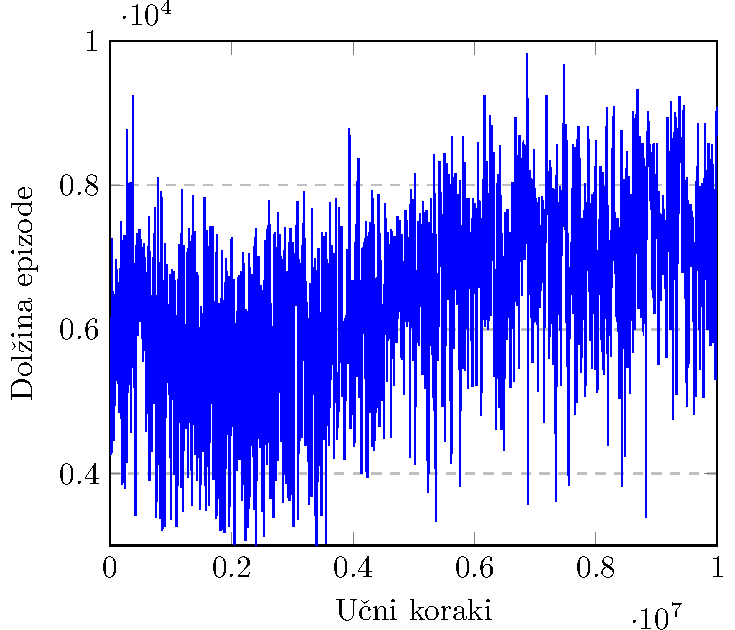
\includegraphics{fig2.pdf}
    \caption{Dolžina epizod glede na število korakov}\label{fig:multiLength}
\end{figure}

Ker pri učenju dveh igralcev enega proti drugem ne moremo uporabiti enakega merila uspešnosti kot pri enoigralskem načinu, smo rezultate prikazali na dva drugačna načina. Kot prvo merilo smo izbrali dolžino posamezne epizode v odvistnosti od števila učnih korakov. Rezultat je prikazan na sliki~\ref{fig:multiLength}. Opazimo lahko, da se dolžina epizode postopoma viša. To je posledica dejstva, da dlje ko se agenta učita, bolje znata odbijati žogo, kar podaljša dolžino epizode (trajanje igre do prejetega ali danega zadetka). Kot drugo merilo uspešnosti igranja smo določili število odbojev žoge posameznega agenta v vsaki epizodi. Rezultati učenja po tem merilu pa so prikazani na sliki~\ref{fig:multiHits}.

\begin{figure}[h]
    \centering
    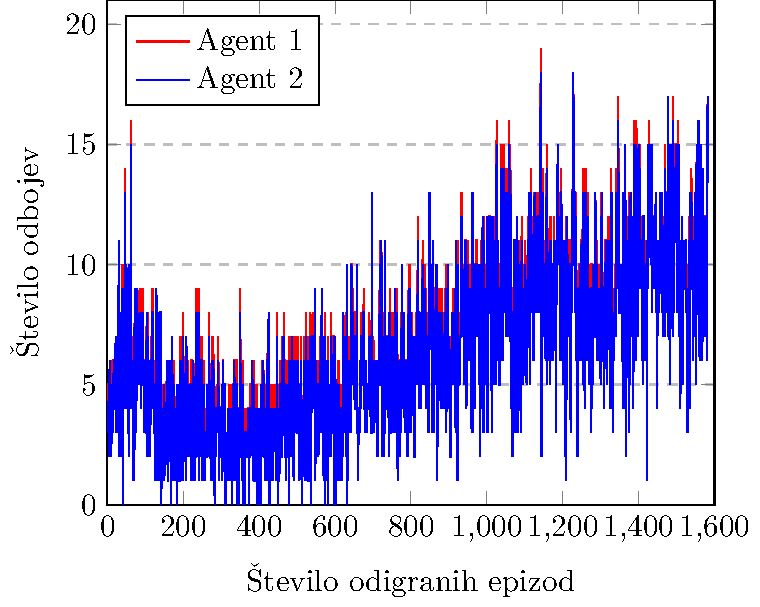
\includegraphics{fig3.pdf}
    \caption{Število odbojev žoge glede na število odigranih epizod}\label{fig:multiHits}
\end{figure}

Opazimo, da se agenta učita približno z enako hitrostjo, kar je pričakovano, saj oba začneta ob enakih začetnih pogojih. Lahko pa vidimo tudi, da ima agent 1 skozi celoten potek učenja nekaj prednosti pred agentom 2, kar je v tem primeru slučajno in posledica začetne sreče agenta 1. 

Rezultate lahko opišemo tudi kvalitativno. Okolje PettingZoo nam omogoča, da lahko potek igre spremljamo v realnem času. To nam omogoča, da lahko razberemo strategije, ki sta se jih nevronski mreži naučili. Na začetku, ko je večina akcij, ki jih nevronski mreži izbereta, naključnih, igralca nimata razvite še nobene strategije. Ko pa izvedeta več učnih korakov, pa postane očitno, da vsaka izmed njiju želi z napadalno strategijo doseči zadetek. Ta strategija je taka, da ko se žoga približuje enemu izmed njiju, jo ta želi odbiti čim bolj z robom loparja, kar povzroči, da se žoga odbije s precej večjo hitrostjo, kot je priletela proti loparju. Ker je žoga odbita z enim izmed robov, je smer odboja vedno proti zgornjem oziroma spodnjem robu igralne površine. Od nje se potem tudi odbije, kar nasprotnika še dodatno zmede in posledično lažje prejme zadetek, saj žoge ne uspe odbiti.

Naučeno napadalno igralno strategijo najlažje ponazorimo z zaporedjem zaslonskih posnetkov, prikazanih na sliki~\ref{fig:screenShots}.

\begin{figure}[H]
    \begin{subfigure}{0.495\linewidth}
        \centering
        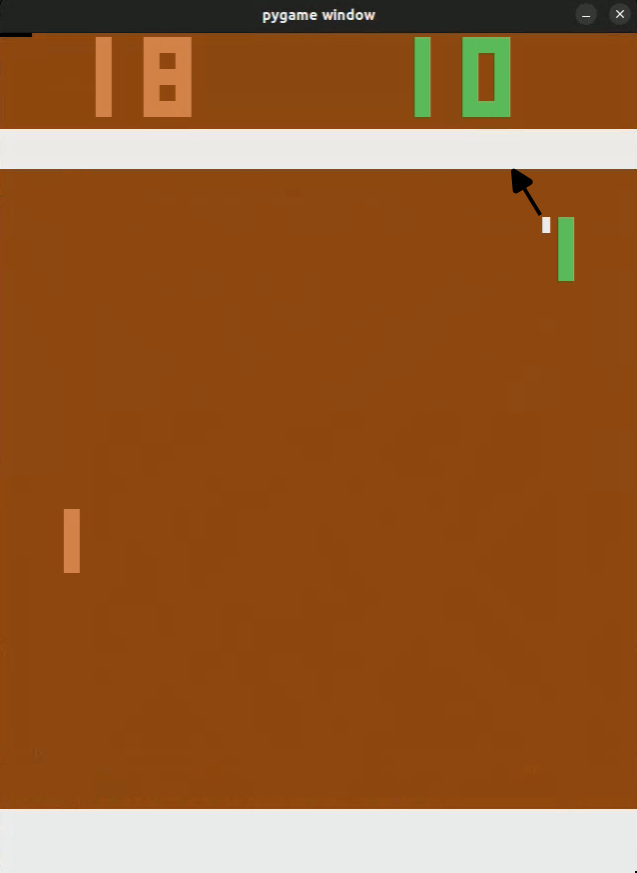
\includegraphics[width=\textwidth]{AttackStrategy.png}
        \caption{Prva zaslonska slika}\label{fig:odbojLoparja}
    \end{subfigure}
    \begin{subfigure}{0.495\linewidth}
        \centering
        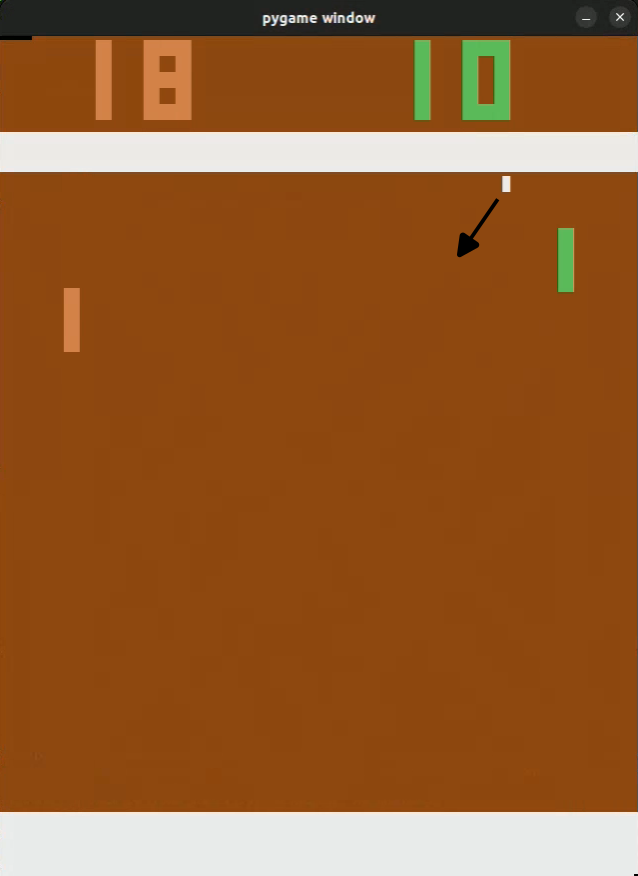
\includegraphics[width=\textwidth]{FirstHit.png}
        \caption{Druga zaslonska slika}\label{fig:firstHit}
    \end{subfigure}
    \begin{subfigure}{0.495\linewidth}
        \centering
        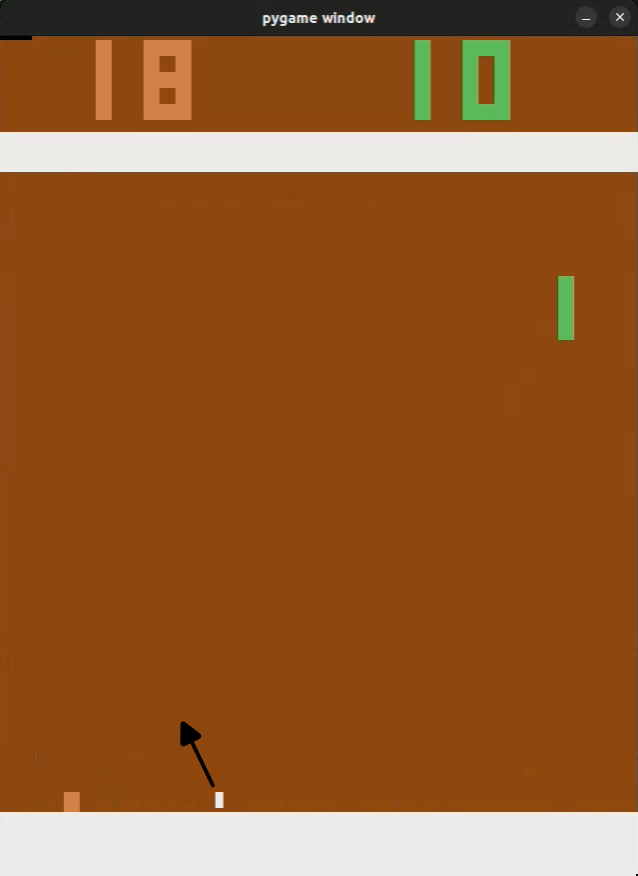
\includegraphics[width=\textwidth]{SecondHit.png}
        \caption{Tretja zaslonska slika}\label{fig:secondHit}
    \end{subfigure}
    \begin{subfigure}{0.495\linewidth}
        \centering
        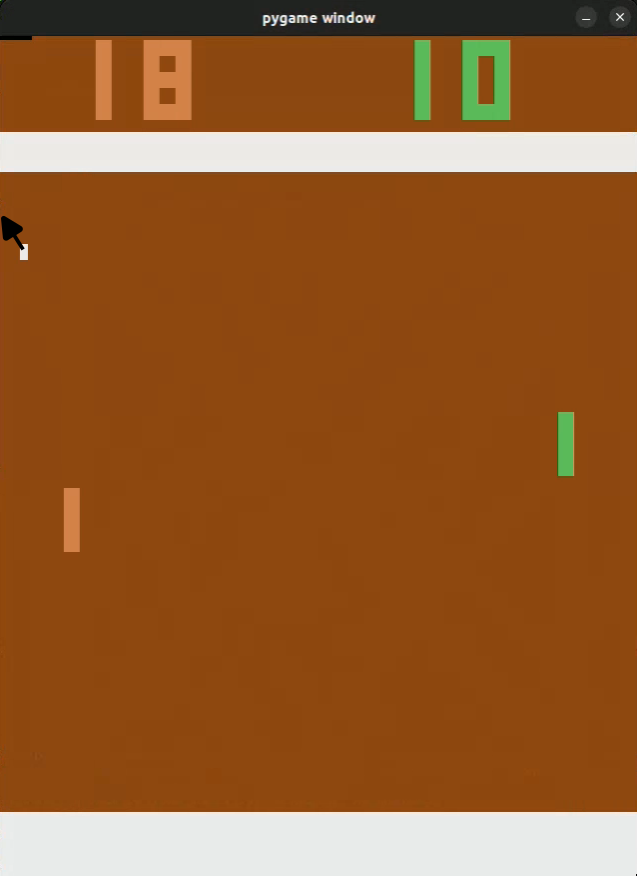
\includegraphics[width=\textwidth]{Score.png}
        \caption{Četrta zaslonska slika}\label{fig:score}
    \end{subfigure}
    \caption{Napadalna igralna strategija. Puščice prikazujejo smer gibanja žogice.}\label{fig:screenShots}
\end{figure}

Desni igralec zelene barve na prvem posnetku~\ref{fig:odbojLoparja} žogo odbije z zgornjim robom loparja, kar mu omogoči, da žogo dobije z večjo močjo. Zato ta dobi pospešek in se odbije od roba igralne površine. Na slikah~\ref{fig:firstHit} in~\ref{fig:secondHit} lahko vidimo, da se je žoga najprej odbila od zgornjega roba igralne površine in potem še od spodnjega, kar je prvega igralca oranžne barve zelo zmedlo in ni vedel, kako naj se postavi, da bo lahko žogo odbil. Posledica tega je slika~\ref{fig:score}, ki prikazuje dosežen zadetek. Prvi igralec je bil pri obrambi neuspešen in je prejel zadetek.

Predstavljeno napadalno strategijo sta razvila oba igralca. Treba je poudariti, da to ne uspeta izvesti prav z vsakim odbojem, temveč to storita nekajkrat med vsako odigrano igro. Če jima to ne uspe, prejmeta zadetek ali pa žogo odbijeta počasi in nasprotniku dopustita dovolj časa, da se pravilno postavi.

\chapter{DISKUSIJA}

V diplomskem delu smo z uporabo arkadnega učnega okolja (ALE) poskušali ugotoviti, kako dobro se lahko dva agenta globokega spodbujevalnega učenja naučita igrati igro Pong na simulaciji igralne konzole Atari 2600, eden proti drugemu. Prostor stanj dvo-igralske različice je bistveno večji od eno-igralske, na kateri je bil DQN demonstriran v preteklosti, zato smo uvedli nekatere prilagoditve --- izločitev konvolucijskih plasti, ki smo jih nadomestili z ročno izluščenimi značilkami iz pomnilnika igralne konzole, ter uvedba pogostejše nagrade. Da bi preiskusili uspešnost svoje prilagojene implementacije globokega spodbujevalnega učenja, smo začeli z implementacijo igre za enega igralca. Algoritem smo pustili igrati 1325 iger proti vgrajenemu igralcu do 5 milijonov učnih korakov, kar je trajalo tri dni na osebnem računalniku. Nadaljevali smo z implementacijo dvoigralskega načina. Algoritmu smo pustili igrati 1583 epizod, kar je trajalo 10 milijonov učnih korakov in približno en teden učenja na istem osebnem računalniku.

Pri enoigralskem načinu so rezultati pokazali, da nevronska mreža konvergira pri 2 milijona učnih korakih. To se zgodi tik preden bi uspela premagati vgrajenega igralca, kar pomeni, da doseže približno enako sposobnost igranja. Če bi povečali arhitekturo skritih plasti te nevronske mreže, bi ta verjetno uspela vgrajenega igralca po zadostnem številu učnih korakov tudi premagati. Uspešnost učenja igre za dva igralca pa smo prikazali na dva nekoliko drugačna načina. Prvi je bil z merjenjem dolžine posamezne epizode. Ta se je višala s številom učnih korakov, kar je posledica uspešnega učenja obrambne strategije. Kot drugo merilo uspešnosti smo šteli število odbojev posamezne nevronske mreže po vsaki odigrani epizodi. Tudi tu so se vrednosti višale s številom učnih korakov, razvidno pa je postalo, da igralca napredujeta približnp enako hitro. V neki epizodi sta igralca dosegla kar 19 in 18 odbojev. Ta najdaljša opažena epizoda je trajala 9835 korakov.

Opazili smo, da sta igralca razvila tudi napadalno strategijo, ki smo jo opisali v poglavju~\ref{section:results}. Ugotovili smo, da sta se igralca naučila, da je potrebno žogo odbiti kar se da z robom loparja, kar povzroči, da se žoga odbije pod ostrim kotom in s povečano hitrostjo. To nasprotnika zmede, saj ta v večini primerov ne zna dovolj hitro prestaviti loparja in preprečiti zadetka.

Pri implementaciji smo imeli največ težav z izbiro primerne arhitekture nevronskih mrež za dvoigralski način. Ker na začetku nismo predvidevali, da je učno okolje za dva igralca precej kompleksnejše od tistega za enega, smo izbirali arhitekture, podobne tistim za enega igralca. To je pripeljalo do tega, da pri učenju nismo bili uspešni in smo na ta način izgubili veliko časa, saj preverjanje vsake konfiguracije vzame veliko časa.

Z opisanimi rezultati smo zadovoljni, saj smo pokazali, da se tudi dva začetniška računalniška igralca uspeta naučiti igro Pong eden proti drugem. Dobljene rezultate bi lahko še izboljšali, če bi arhitekture skritih plasti nevronskih mrež še povečali, a bi se s tem čas učenja podaljšal preko procesnih zmogljivosti, ki smo jih imeli na voljo. To zato ostaja kot možnost za nadaljnje delo. Zanimivo bi bilo tudi preiskusiti, kako dobro bi se naučena igralca iz dvo-igralskega okolja obnesla v eno-igralskem okolju. Zanimalo bi nas, če sta se naučila dovolj splošne strategije igranja, da bi lahko obvladala vgrajeni igralni algoritem. Še zanimivejše pa bi bilo namesto vgrajenega igralca nasproti igralcema iz dvoigralskega načina postaviti človeka. Izpeljali bi turnir, na katerem bi ljudje igrali proti naučenima agentoma. Na podlagi rezultatov bi ugotavljali, če sta naučena agenta dosegla ali celo presegla človeški nivo igranja igre.

\end{document}